%%%%%%%%%%%%%%%%%%%%%%%%%%%%%%%%%%%%%%%%%%%%%%%%%%%%%%%%%%%%%%%%%%%%%%%%%%%%
% AGUtmpl.tex: this template file is for articles formatted with LaTeX2e,
% Modified November 2013
%
% This template includes commands and instructions
% given in the order necessary to produce a final output that will
% satisfy AGU requirements.
%
% PLEASE DO NOT USE YOUR OWN MACROS
% DO NOT USE \newcommand, \renewcommand, or \def.
%
% FOR FIGURES, DO NOT USE \psfrag
%
%%%%%%%%%%%%%%%%%%%%%%%%%%%%%%%%%%%%%%%%%%%%%%%%%%%%%%%%%%%%%%%%%%%%%%%%%%%%
%
% All questions should be e-mailed to latex@agu.org.
%
%%%%%%%%%%%%%%%%%%%%%%%%%%%%%%%%%%%%%%%%%%%%%%%%%%%%%%%%%%%%%%%%%%%%%%%%%%%%
%
% Step 1: Set the \documentclass
%
% There are two options for article format: two column (default)
% and draft.
%
% PLEASE USE THE DRAFT OPTION TO SUBMIT YOUR PAPERS.
% The draft option produces double spaced output.
%
% Choose the journal abbreviation for the journal you are
% submitting to:

% jgrga JOURNAL OF GEOPHYSICAL RESEARCH
% gbc   GLOBAL BIOCHEMICAL CYCLES
% grl   GEOPHYSICAL RESEARCH LETTERS
% pal   PALEOCEANOGRAPHY
% ras   RADIO SCIENCE
% rog   REVIEWS OF GEOPHYSICS
% tec   TECTONICS
% wrr   WATER RESOURCES RESEARCH
% gc    GEOCHEMISTRY, GEOPHYSICS, GEOSYSTEMS
% sw    SPACE WEATHER
% ms    JAMES
% ef    EARTH'S FUTURE
%
%
%
% (If you are submitting to a journal other than jgrga,
% substitute the initials of the journal for "jgrga" below.)

\documentclass[draft,jgrga]{agutexSI}



%%%%%%%%%%%%%%%%%%%%%%%%%%%%%%%%%%%%%%%%%%%%%%%%%%%%%%%%%%%%%%%%%%%%%%%%%
%
%  SUPPORTING INFORMATION TEMPLATE
%
%% ------------------------------------------------------------------------ %%
%
%
%Please use this template when formatting and submitting your Supporting Information.

%This template serves as both a “table of contents” for the supporting information for your article and as a summary of files.
%
%
%OVERVIEW
%
%Please note that all supporting information will be peer reviewed with your manuscript.
%In general, the purpose of the supporting information is to enable authors to provide and archive auxiliary information such as data %tables, method information, figures, video, or computer software, in digital formats so that other scientists can use it.
%The key criteria are that the data:
% 1. supplement the main scientific conclusions of the paper but are not essential to the conclusions (with the exception of
%    including %data so the experiment can be reproducible);
% 2. are likely to be usable or used by other scientists working in the field;
% 3. are described with sufficient precision that other scientists can understand them, and
% 4. are not exe files.
%
%USING THIS TEMPLATE
%
%***All references should be included in the reference list of the main paper so that they can be indexed, linked, and counted as citations.  The reference section does not count toward length limits.
%
%All Supporting text and figures should be included in this document. Insert supporting information content into each appropriate section of the template. %Figures and tables should appear above each caption.  To add additional captions, simply copy and paste each sample caption as needed.

%Tables may be included, but can also be uploaded separately, especially if they are larger than 1 page, or if necessary for retaining table formatting. Data sets, large tables, movie files, and audio files should be uploaded separately, following AGU naming conventions. Include their captions in this document and list the file name with the caption. You will be prompted to upload these files on the Upload Files tab during the submission process, using file type “Supporting Information (SI)”

%IMPORTANT NOTE ON FIGURES AND TABLES
% Placeholders for figures and tables appear after the \end{article} command, after references.
% DO NOT USE \psfrag or \subfigure commands.
%
%  Uncomment the following command to include .eps files
 \usepackage{graphicx}
%
%  Uncomment the following command to allow illustrations to print
%   when using Draft:
\setkeys{Gin}{draft=false}
%
% Substitute one of the following for [dvips] above
% if you are using a different driver program and want to
% proof your illustrations on your machine:
%
% [xdvi], [dvipdf], [dvipsone], [dviwindo], [emtex], [dviwin],
% [pctexps],  [pctexwin],  [pctexhp],  [pctex32], [truetex], [tcidvi],
% [oztex], [textures]
%
%
%% ------------------------------------------------------------------------ %%
%
%  ENTER PREAMBLE
%
%% ------------------------------------------------------------------------ %%

% Author names in capital letters:
\authorrunninghead{PINNINGTON ET AL.}

% Shorter version of title entered in capital letters:
\titlerunninghead{USING DATA ASSIMILATION TO UNDERSTAND DISTURBANCE}

%Corresponding author mailing address and e-mail address:
\authoraddr{Corresponding author: E. M. Pinnington,
(e.m.pinnington@pgr.reading.ac.uk)}

\begin{document}

%% ------------------------------------------------------------------------ %%
%
%  TITLE
%
%% ------------------------------------------------------------------------ %%

%\includegraphics{agu_pubart-white_reduced.eps}


\title{Supporting Information for ``Using data assimilation to understand the effect of disturbance on the carbon dynamics of a managed woodland"}
%
% e.g., \title{Supporting Information for "Terrestrial ring current:
% Origin, formation, and decay $\alpha\beta\Gamma\Delta$"}
%
%DOI: 10.1002/%insert paper number here%

%% ------------------------------------------------------------------------ %%
%
%  AUTHORS AND AFFILIATIONS
%
%% ------------------------------------------------------------------------ %%


%Use \author{\altaffilmark{}} and \altaffiltext{}

% \altaffilmark will produce footnote;
% matching \altaffiltext will appear at bottom of page.

% \authors{A. B. Smith,\altaffilmark{1}
% Eric Brown,\altaffilmark{1,2} Rick Williams,\altaffilmark{3}
% John B. McDougall\altaffilmark{4}, and S. Visconti\altaffilmark{5}}

%\altaffiltext{1}{Department of Hydrology and Water Resources,
%University of Arizona, Tucson, Arizona, USA.}

%\altaffiltext{2}{Department of Geography, Ohio State University,
%Columbus, Ohio, USA.}

%\altaffiltext{3}{Department of Space Sciences, University of
%Michigan, Ann Arbor, Michigan, USA.}

%\altaffiltext{4}{Division of Hydrologic Sciences, Desert Research
%Institute, Reno, Nevada, USA.}

%\altaffiltext{5}{Dipartimento di Idraulica, Trasporti ed
%Infrastrutture Civili, Politecnico di Torino, Turin, Italy.}

\authors{Ewan M. Pinnington,\altaffilmark{1}
Eric Casella,\altaffilmark{3} Sarah L. Dance,\altaffilmark{1,2} Amos S. Lawless,\altaffilmark{1,2,4}
James I. L. Morison,\altaffilmark{3} Nancy K. Nichols,\altaffilmark{1,2,4} Matthew Wilkinson,\altaffilmark{3}
Tristan L. Quaife,\altaffilmark{1,4}}


% \affiliation{1}{First Affiliation}
% \affiliation{2}{Second Affiliation}
% \affiliation{3}{Third Affiliation}
% \affiliation{4}{Fourth Affiliation}

\altaffiltext{1}{Department of Meteorology, University of Reading, Reading, UK}
\altaffiltext{2}{Department of Mathematics and Statistics, University of Reading, Reading, UK}
\altaffiltext{3}{Centre for Sustainable Forestry and Climate Change, Forest Research, Alice Holt, Farnham, UK}
\altaffiltext{4}{National Centre for Earth Observation, University of Reading, Reading, UK}

%% ------------------------------------------------------------------------ %%
%
%  BEGIN ARTICLE
%
%% ------------------------------------------------------------------------ %%

% The body of the article must start with a \begin{article} command
%
% \end{article} must follow the references section, before the figures
%  and tables.

\begin{article}

%% ------------------------------------------------------------------------ %%
%
%  TEXT
%
%% ------------------------------------------------------------------------ %%



\noindent\textbf{Contents of this file}
%%%Remove or add items as needed%%%
\begin{enumerate}
\item Table S1
\item Figures S1 to S12
%if Tables are larger than 1 page, upload as separate excel file
\end{enumerate}


\noindent\textbf{Introduction}
%Type or paste your text here. The introduction gives a brief overview of the supporting information. You should include information %about as many of the following as possible (when appropriate):
% 1. a general overview of the kind of data files;
% 2. information about when and how the data were collected or created;
% 3. a general description of processing steps used;
% 4. any known imperfections or anomalies in the data.

In Figures S1-S10 we present extra plots from the three experiments outlined in the paper (A, B \& C), we also add plots for a fourth experiment (labelled experiment D here) where only LAI, leaf mass per area and woody biomass are assimilated with the DALEC2 model. The summary statistics for experiment D are also included in table~\ref{table:sum_stats}.

In Figure S11 we show the prior model trajectory and observations of daytime NEE for 2012-2013, this is the period in which the prior model was calibrated.

Figure S12 shows phenocam observations of green fraction taken at the Alice Holt flux site, The LAI as predicted by experiment C is also shown o this figure.
%\clearpage

%Delete all unused file types below. Copy/paste for multiples of each file type as needed.
%\noindent\textbf{Text S1.}
%Type or paste text here. This should be additional explanatory text, such as: extended descriptions of results, full details of models, extended lists of acknowledgements etc.  It should not be additional discussion, analysis, interpretation or critique. It should not be an additional scientific experiment or paper.
%
%Repeat for any additional Supporting Text

%%Enter Data Set, Movie, and Audio captions here
%%EXAMPLE CAPTIONS

%\noindent\textbf{Table S1.} %Type or paste caption here.
%upload your dataset(s) to AGU's journal submission site and select "Supporting Information (SI)" as the file type. Following naming %convention: ds01.

%Repeat for any additional Supporting data sets

%\noindent\textbf{Movie S1.} %Type or paste caption here.
%upload your movie(s) to AGU's journal submission site and select, "Supporting Information %(SI)" as the file type. Following naming convention: ms01.

%Repeat any additional Supporting movies

%\noindent\textbf{Audio S1.} %Type or paste caption here.
%upload your audio file(s) to AGU's journal submission site and select "Supporting Information %(SI)" as the file type. Following naming convention: auds01.

%Repeat for any additional Supporting audio files

%%% End of body of article:
%%%%%%%%%%%%%%%%%%%%%%%%%%%%%%%%%%%%%%%%%%%%%%%%%%%%%%%%%%%%%%%%
%
% Optional Notation section goes here
%
% Notation -- End each entry with a period.
% \begin{notation}
% Term & definition.\\
% Second term & second definition.\\
% \end{notation}
%%%%%%%%%%%%%%%%%%%%%%%%%%%%%%%%%%%%%%%%%%%%%%%%%%%%%%%%%%%%%%%%


%% ------------------------------------------------------------------------ %%
%%  REFERENCE LIST AND TEXT CITATIONS
%
% Either type in your references using
% \begin{thebibliography}{}
% \bibitem{}
% Text
% \end{thebibliography}
%
% Or,
%
% If you use BiBTeX for your references, please use the agufull08.bst file (available at % ftp://ftp.agu.org/journals/latex/journals/Manuscript-Preparation/) to produce your .bbl
% file and copy the contents into your paper here.
%
% Follow these steps:
% 1. Run LaTeX on your LaTeX file.
%
% 2. Make sure the bibliography style appears as \bibliographystyle{agufull08}. Run BiBTeX on your LaTeX
% file.
\bibliographystyle{agufull08}
\bibliography{../../PhD.bib}
%
% 3. Open the new .bbl file containing the reference list and
%   copy all the contents into your LaTeX file here.
%
% 4. Comment out the old \bibliographystyle and \bibliography commands.
%
% 5. Run LaTeX on your new file before submitting.
%
% AGU does not want a .bib or a .bbl file. Please copy in the contents of your .bbl file here.

%\begin{thebibliography}{}

%\providecommand{\natexlab}[1]{#1}
%\expandafter\ifx\csname urlstyle\endcsname\relax
%  \providecommand{\doi}[1]{doi:\discretionary{}{}{}#1}\else
%  \providecommand{\doi}{doi:\discretionary{}{}{}\begingroup
%  \urlstyle{rm}\Url}\fi
%
%\bibitem[{\textit{Atkinson and Sloan}(1991)}]{AtkinsonSloan}
%Atkinson, K., and I.~Sloan (1991), The numerical solution of first-kind
%  logarithmic-kernel integral equations on smooth open arcs, \textit{Math.
%  Comp.}, \textit{56}(193), 119--139.
%
%\bibitem[{\textit{Colton and Kress}(1983)}]{ColtonKress1}
%Colton, D., and R.~Kress (1983), \textit{Integral Equation Methods in
%  Scattering Theory}, John Wiley, New York.
%
%\bibitem[{\textit{Hsiao et~al.}(1991)\textit{Hsiao, Stephan, and
%  Wendland}}]{StephanHsiao}
%Hsiao, G.~C., E.~P. Stephan, and W.~L. Wendland (1991), On the {D}irichlet
%  problem in elasticity for a domain exterior to an arc, \textit{J. Comput.
%  Appl. Math.}, \textit{34}(1), 1--19.
%
%\bibitem[{\textit{Lu and Ando}(2012)}]{LuAndo}
%Lu, P., and M.~Ando (2012), Difference of scattering geometrical optics
%  components and line integrals of currents in modified edge representation,
%  \textit{Radio Sci.}, \textit{47},  RS3007, \doi{10.1029/2011RS004899}.

%\end{thebibliography}

%Reference citation examples:

%...as shown by \textit{Kilby} [2008].
%...as shown by {\textit  {Lewin}} [1976], {\textit  {Carson}} [1986], {\textit  {Bartholdy and Billi}} [2002], and {\textit  {Rinaldi}} [2003].
%...has been shown [\textit{Kilby et al.}, 2008].
%...has been shown [{\textit  {Lewin}}, 1976; {\textit  {Carson}}, 1986; {\textit  {Bartholdy and Billi}}, 2002; {\textit  {Rinaldi}}, 2003].
%...has been shown [e.g., {\textit  {Lewin}}, 1976; {\textit  {Carson}}, 1986; {\textit  {Bartholdy and Billi}}, 2002; {\textit  {Rinaldi}}, 2003].

%...as shown by \citet{jskilby}.
%...as shown by \citet{lewin76}, \citet{carson86}, \citet{bartoldy02}, and \citet{rinaldi03}.
%...has been shown \citep{jskilbye}.
%...has been shown \citep{lewin76,carson86,bartoldy02,rinaldi03}.
%...has been shown \citep [e.g.,][]{lewin76,carson86,bartoldy02,rinaldi03}.
%
% Please use ONLY \citet and \citep for reference citations.
% DO NOT use other cite commands (e.g., \cite, \citeyear, \nocite, \citealp, etc.).

%% ------------------------------------------------------------------------ %%
%
%  END ARTICLE
%
%% ------------------------------------------------------------------------ %%
\end{article}
\clearpage

% Delete all unused file types below. Copy/paste for multiples of each file type as needed.

% enter figures and tables here:
%
% EXAMPLE FIGURE
% ---------------
% \begin{figure}
%\setfigurenum{S1} %%Change number for each figure
% \noindent\includegraphics[width=20pc]{samplefigure.eps}
%\caption{Caption text here}
 %\label{figure_label}
 %\end{figure}
 
\begin{figure}
\setfigurenum{S1} %%Change number for each figure
 \noindent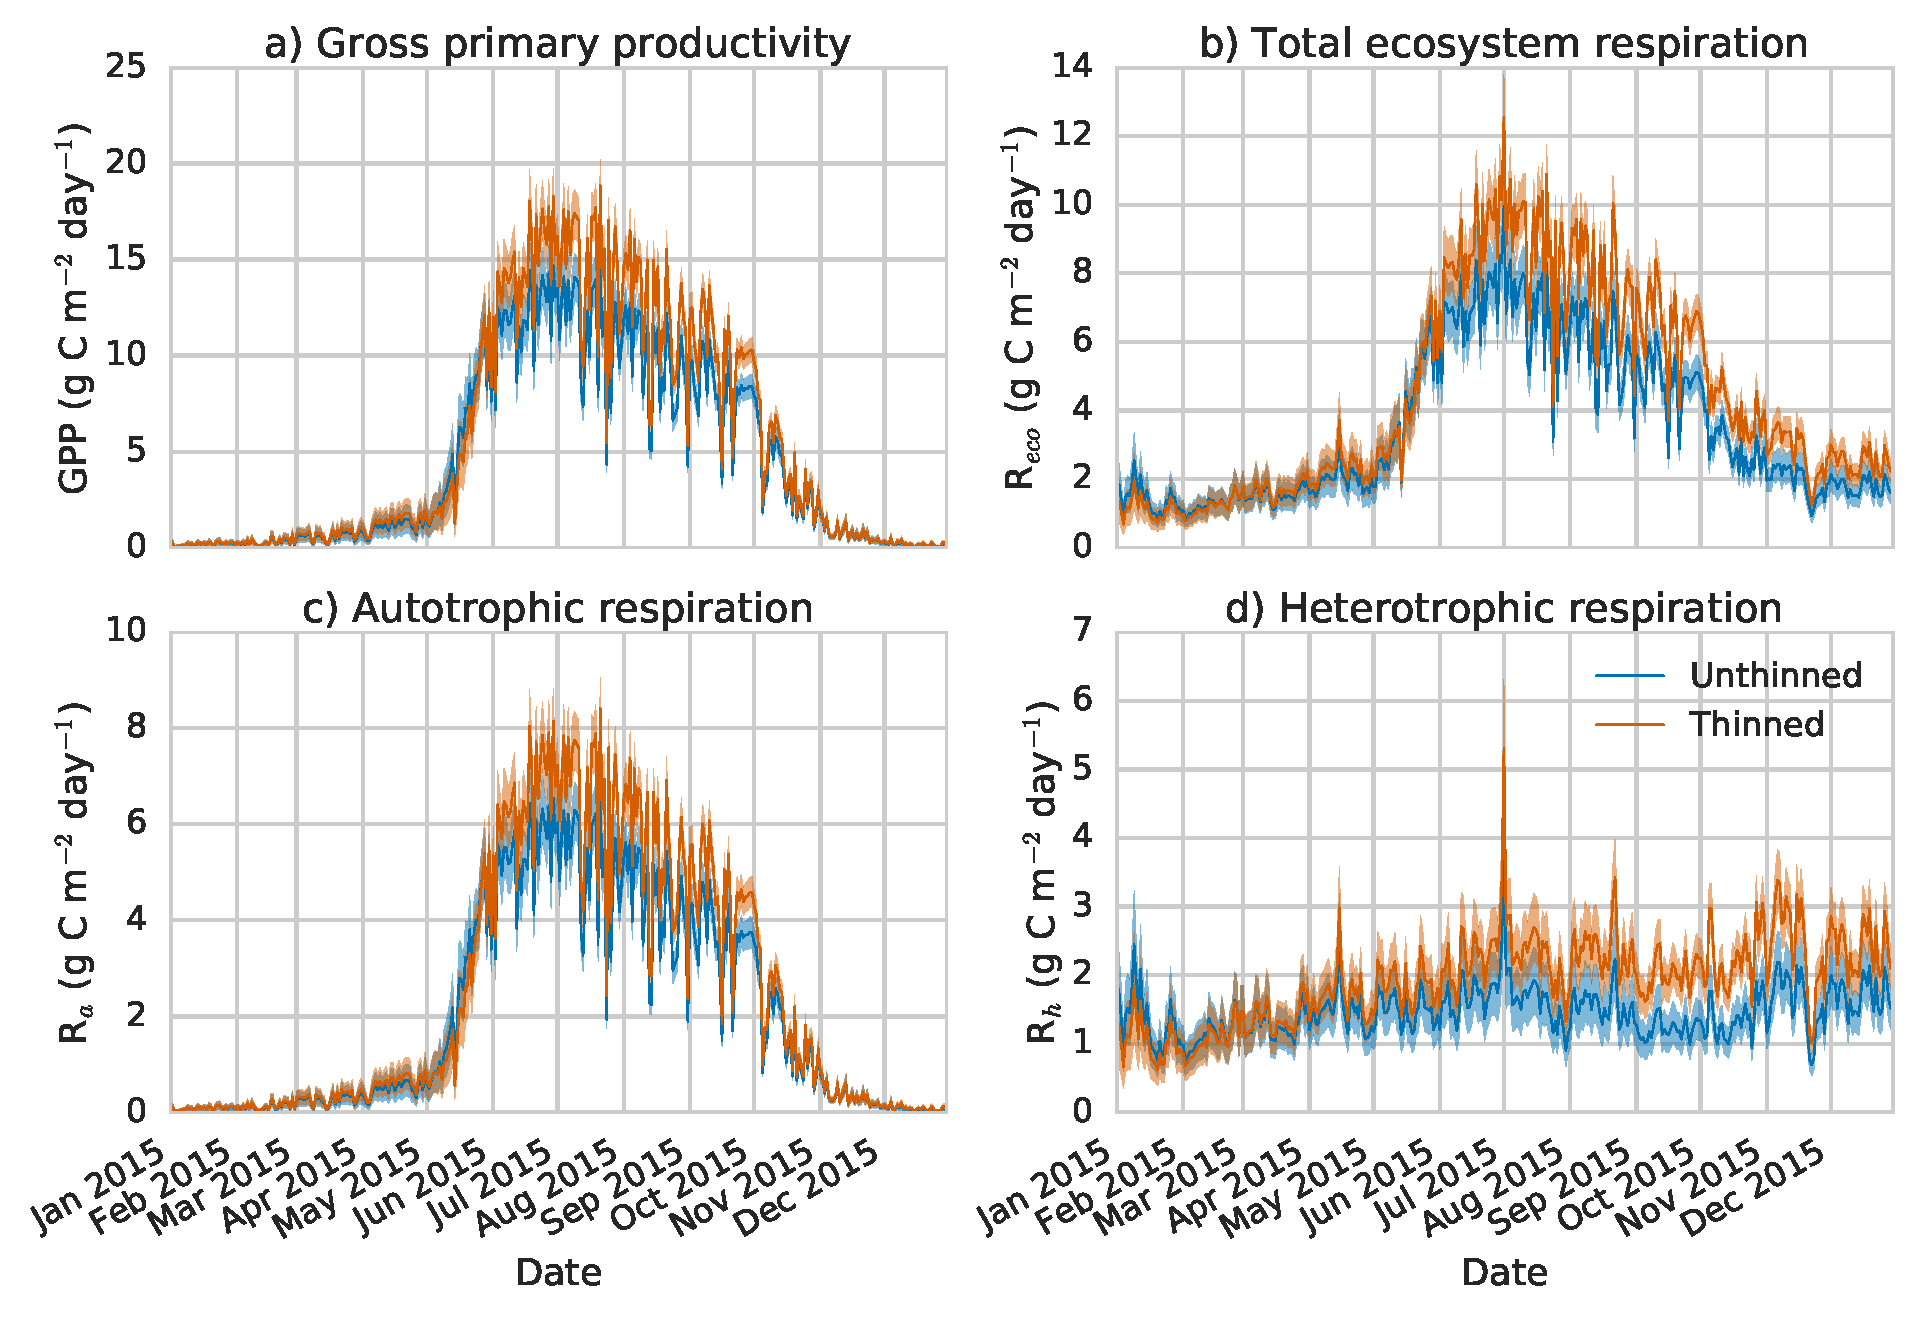
\includegraphics[width=40pc]{flux_compa.pdf}
\caption{Experiment A: 2015 unthinned and thinned forest model trajectories after assimilation. Blue line: model trajectory after assimilation of unthinned forest data, blue shading: uncertainty in model trajectory after assimilation (\(\pm\) 1 standard deviation), orange line: model trajectory after assimilation of thinned forest data, orange shading: uncertainty in model trajectory after assimilation (\(\pm\) 1 standard deviation).}
 \label{fig:fluxcompa}
 \end{figure}
 
 \begin{figure}
\setfigurenum{S2} %%Change number for each figure
 \noindent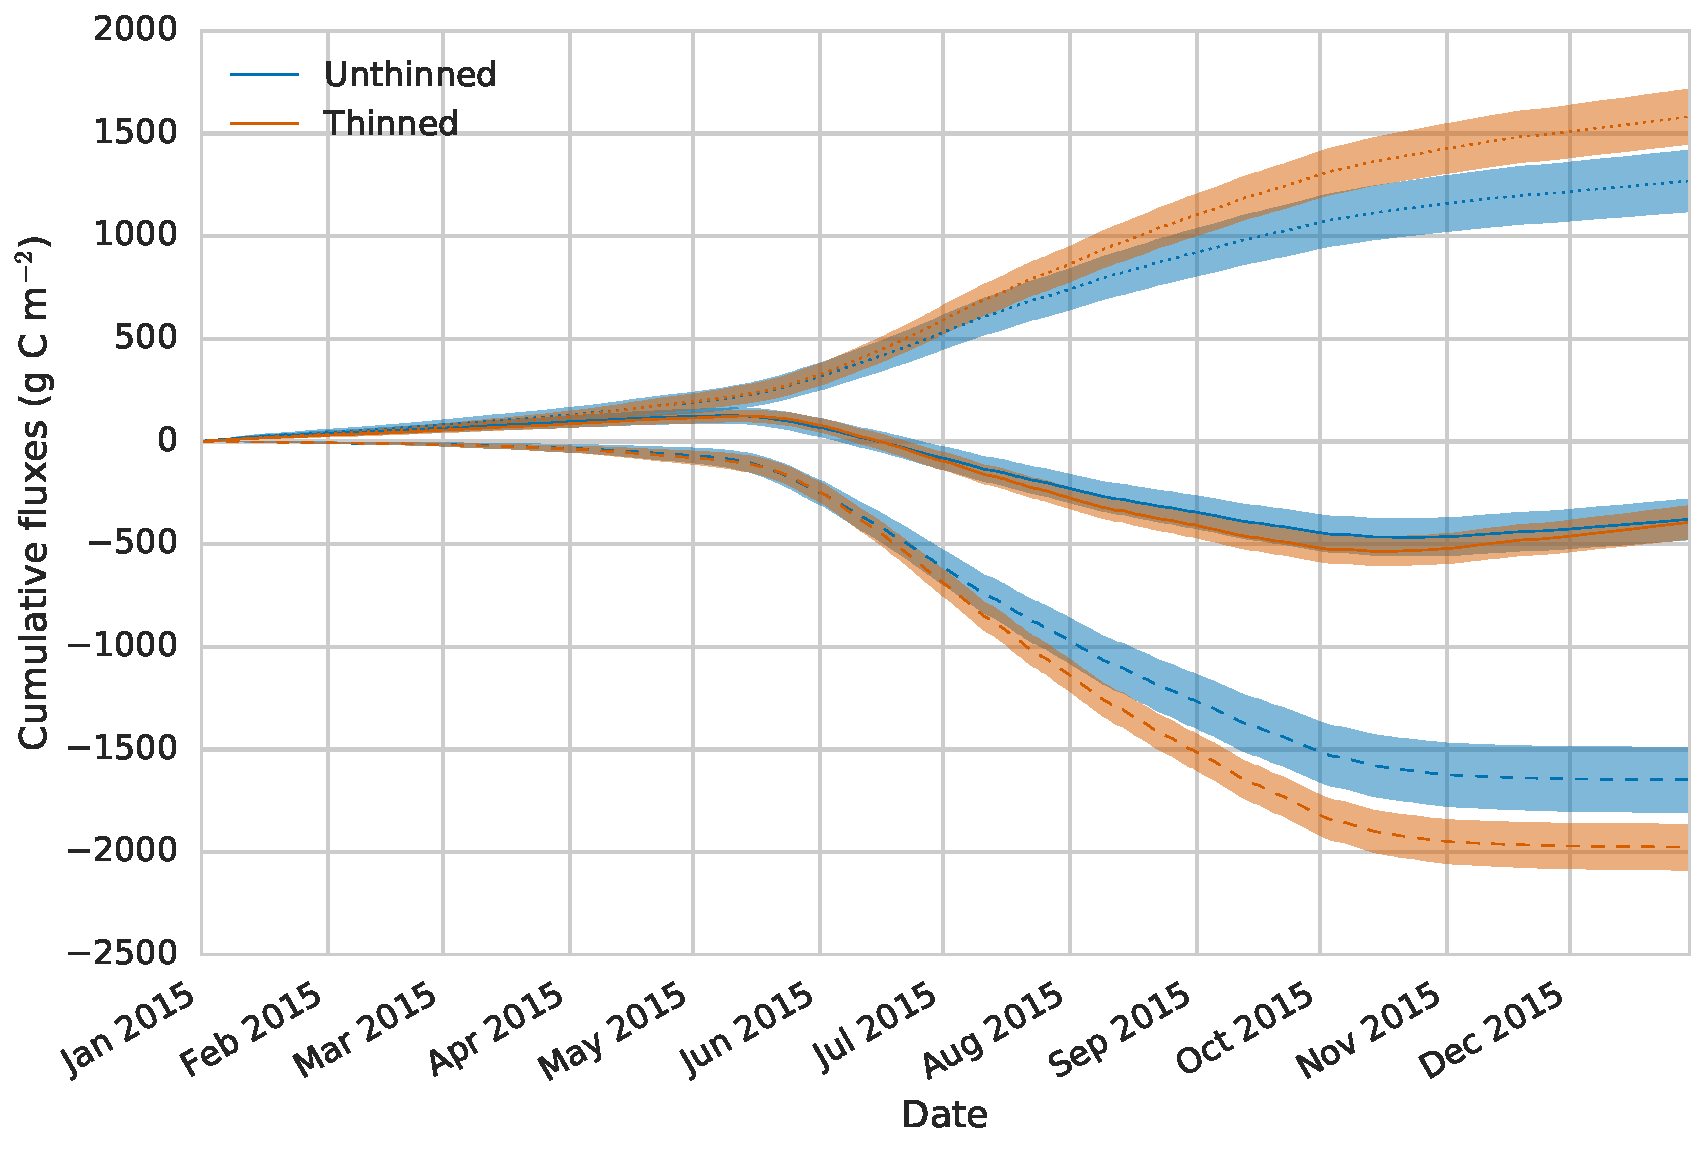
\includegraphics[width=40pc]{cum_fluxa.pdf}
\caption{Experiment A: 2015 unthinned and thinned forest model trajectories for cumulative fluxes after assimilation. Solid line cumulative NEE, dotted line: cumulative ecosystem respiration, dashed line: cumulative GPP (NEE=-GPP+RT). Colour and shading has the same meaning as in Figure~\ref{fig:fluxcompa}.}
 \label{fig:fluxcuma}
 \end{figure}


 \begin{figure}
\setfigurenum{S3} %%Change number for each figure
 \noindent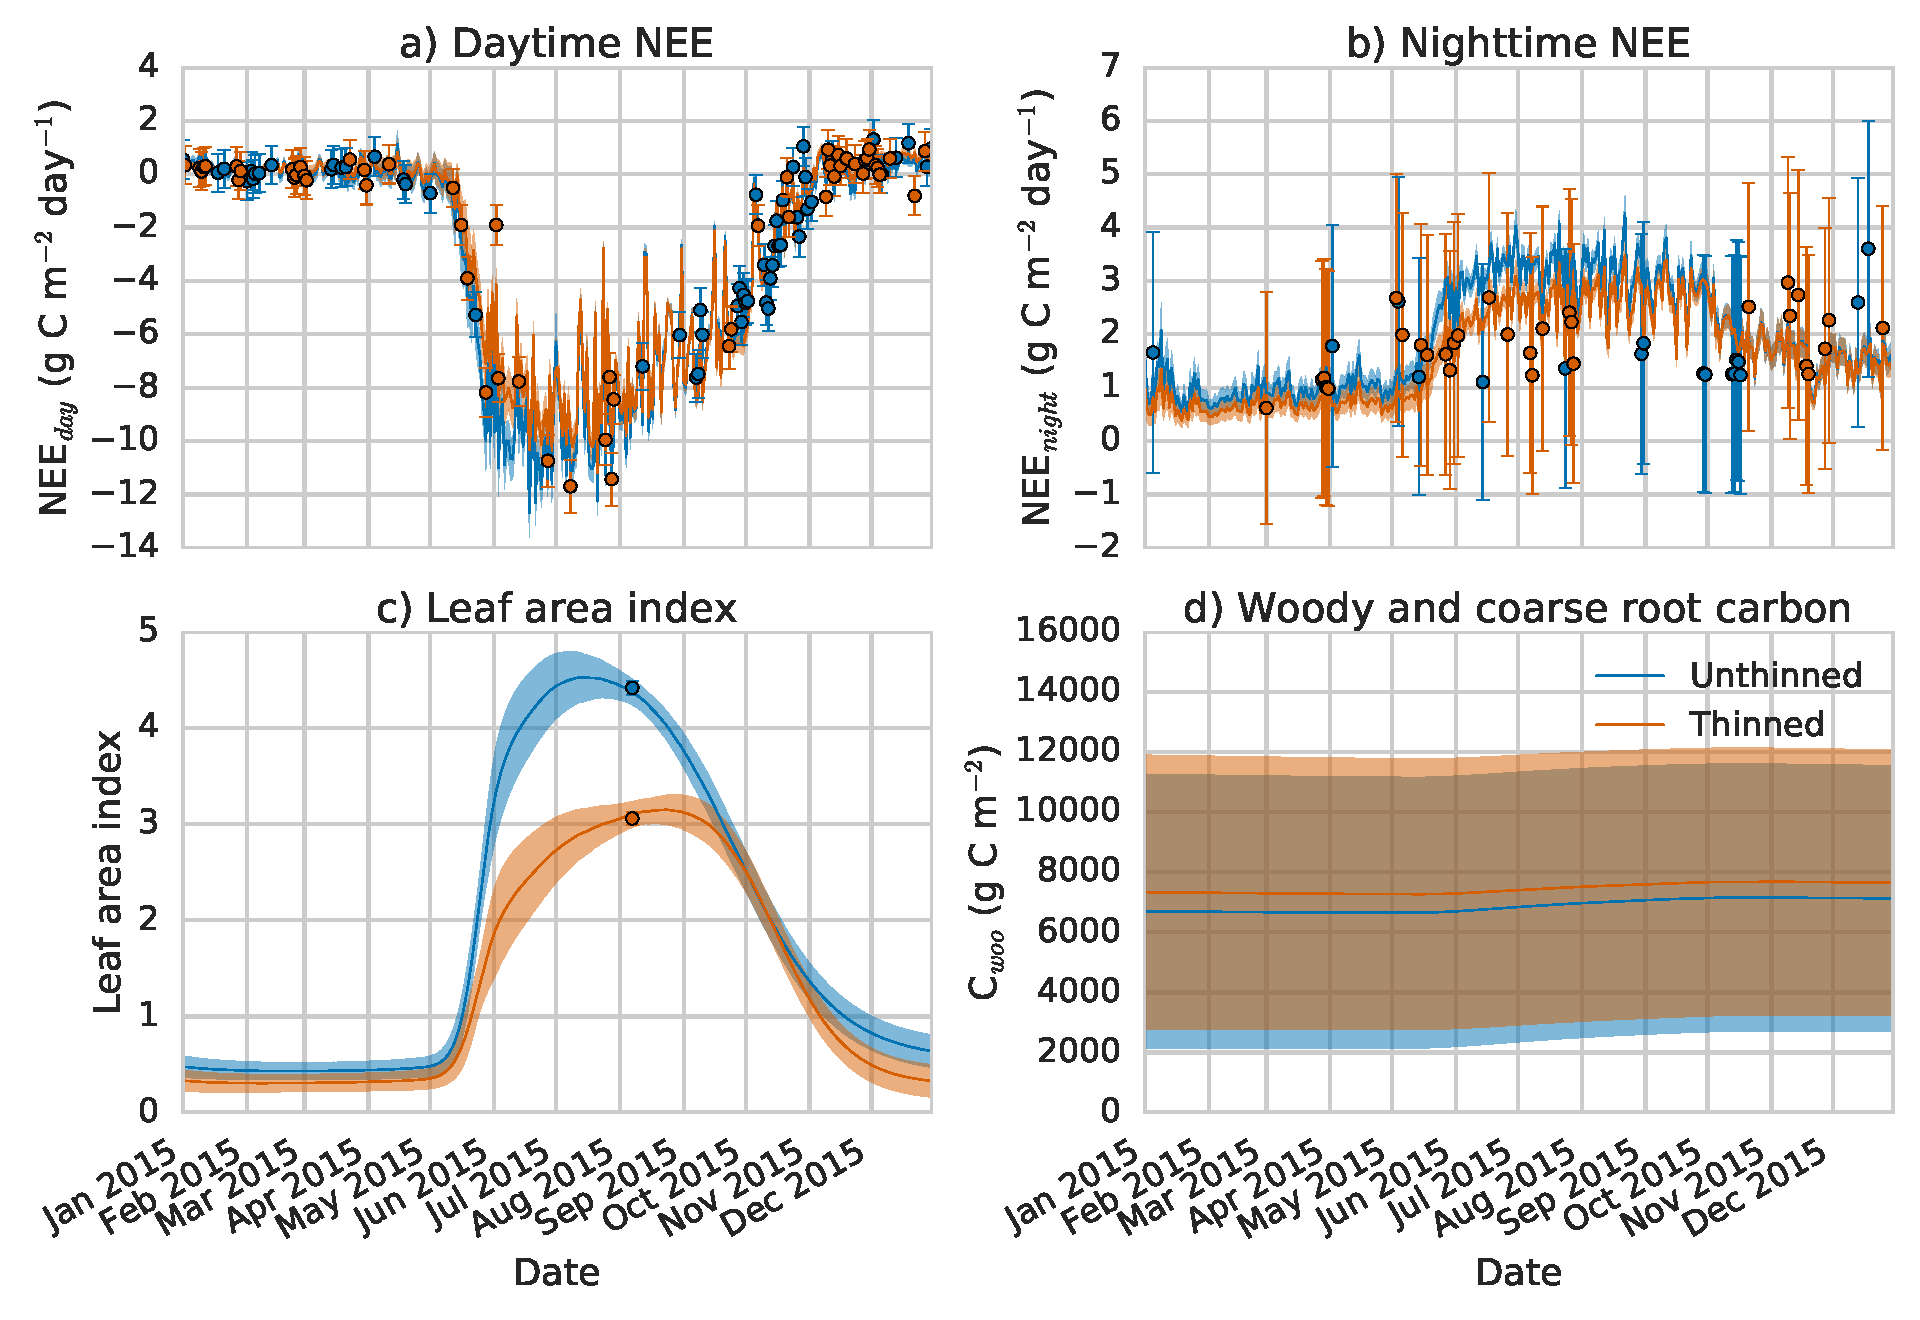
\includegraphics[width=40pc]{obs_compb.pdf}
\caption{Experiment B: 2015 unthinned and thinned forest observations and model trajectories after assimilation. Blue line: model trajectory after assimilation of unthinned data, blue shading: uncertainty in model trajectory after assimilation (\(\pm\) 1 standard deviation), blue dots: unthinned observations with error bars, orange line: model trajectory after assimilation of thinned data, orange shading: uncertainty in model trajectory after assimilation (\(\pm\) 1 standard deviation), orange dots: thinned observations with error bars.}
 \label{fig:obscompb}
 \end{figure}
 
 
 \begin{figure}
\setfigurenum{S4} %%Change number for each figure
 \noindent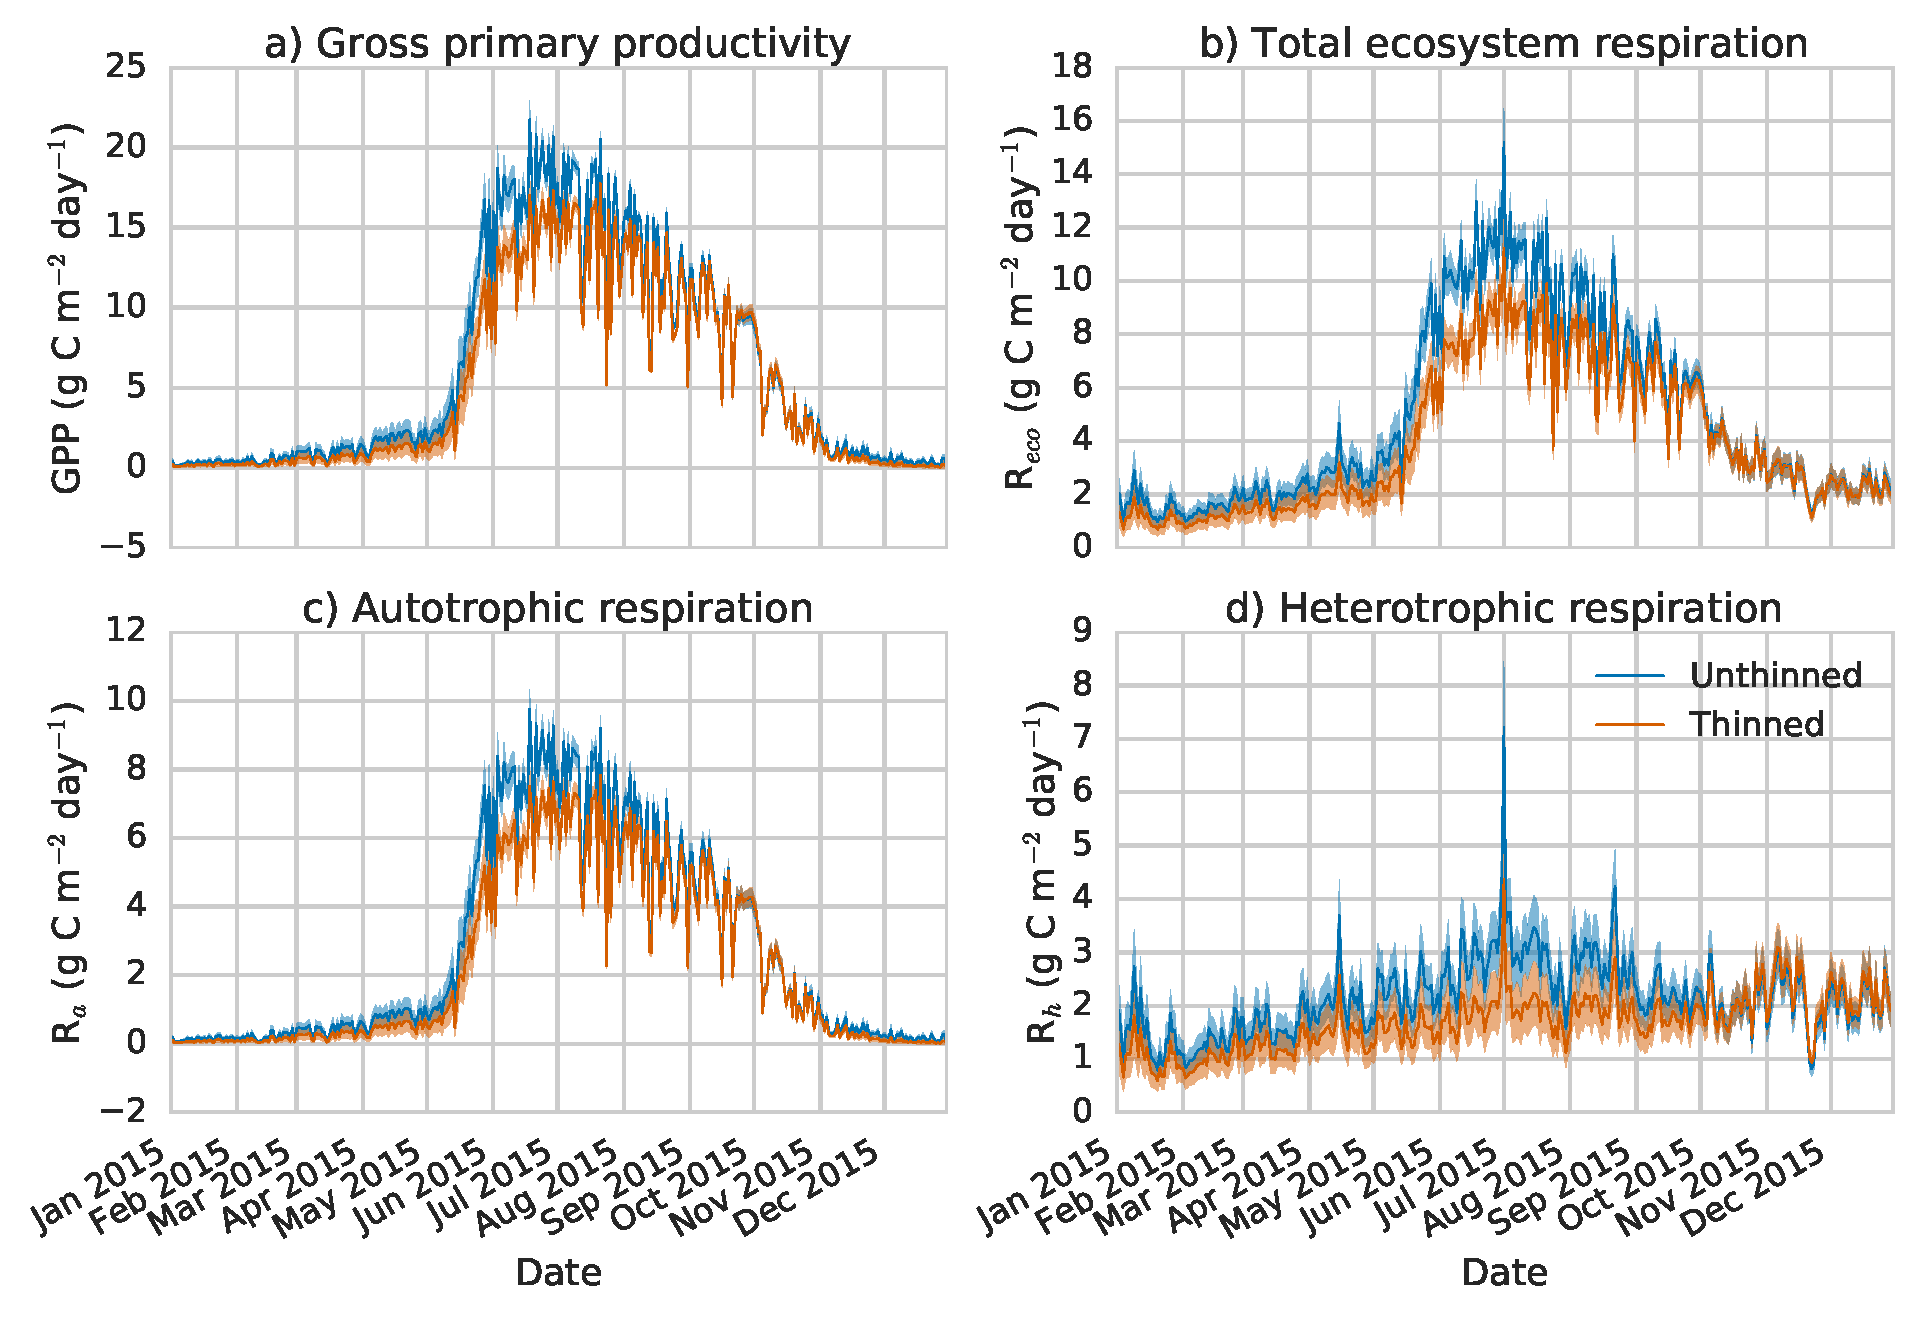
\includegraphics[width=40pc]{flux_compb.pdf}
\caption{Experiment B: 2015 unthinned and thinned forest model trajectories after assimilation. Colour and shading has the same meaning as in Figure~\ref{fig:fluxcompa}.}
 \label{fig:fluxcompb}
 \end{figure}
 
  \begin{figure}
\setfigurenum{S5} %%Change number for each figure
 \noindent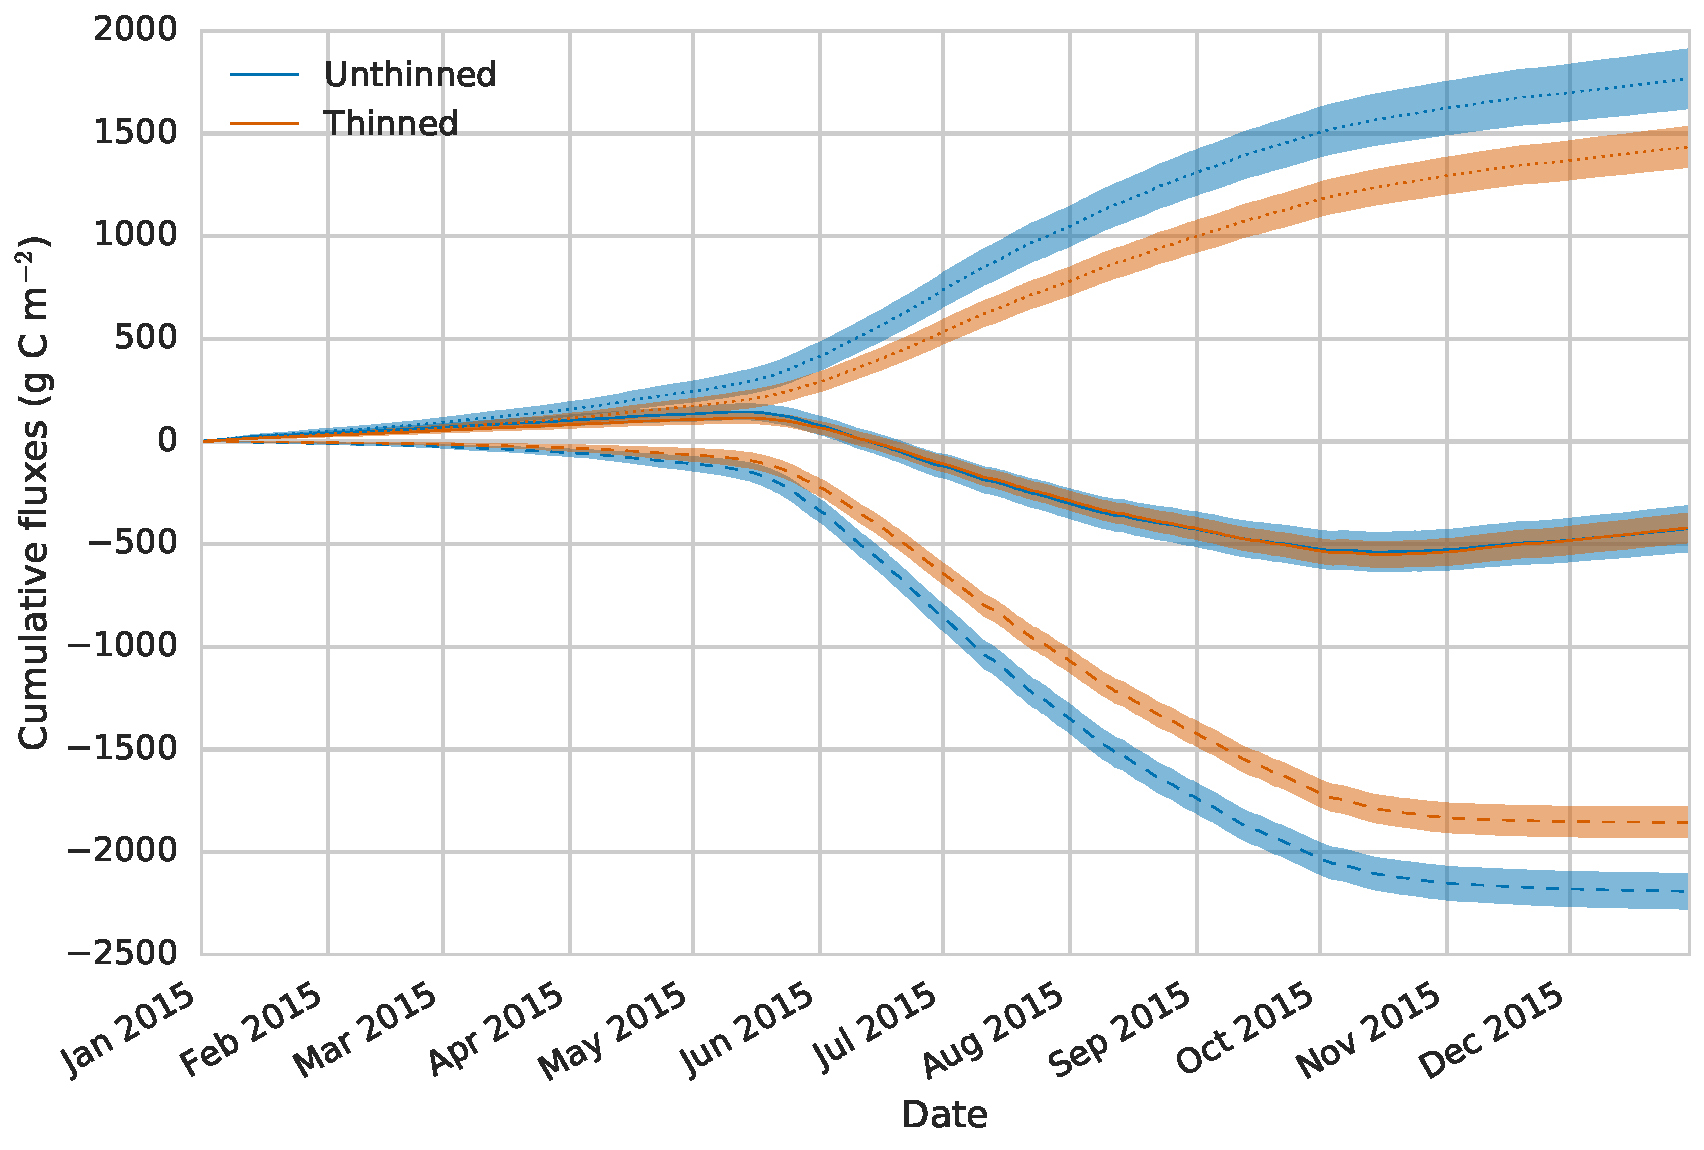
\includegraphics[width=40pc]{cum_fluxb.pdf}
\caption{Experiment B: 2015 unthinned and thinned forest model trajectories for cumulative fluxes after assimilation. Solid line cumulative NEE, dotted line: cumulative ecosystem respiration, dashed line: cumulative GPP (NEE=-GPP+RT). Colour and shading has the same meaning as in Figure~\ref{fig:fluxcompa}.}
 \label{fig:fluxcumb}
 \end{figure}
 
  \begin{figure}
\setfigurenum{S6} %%Change number for each figure
 \noindent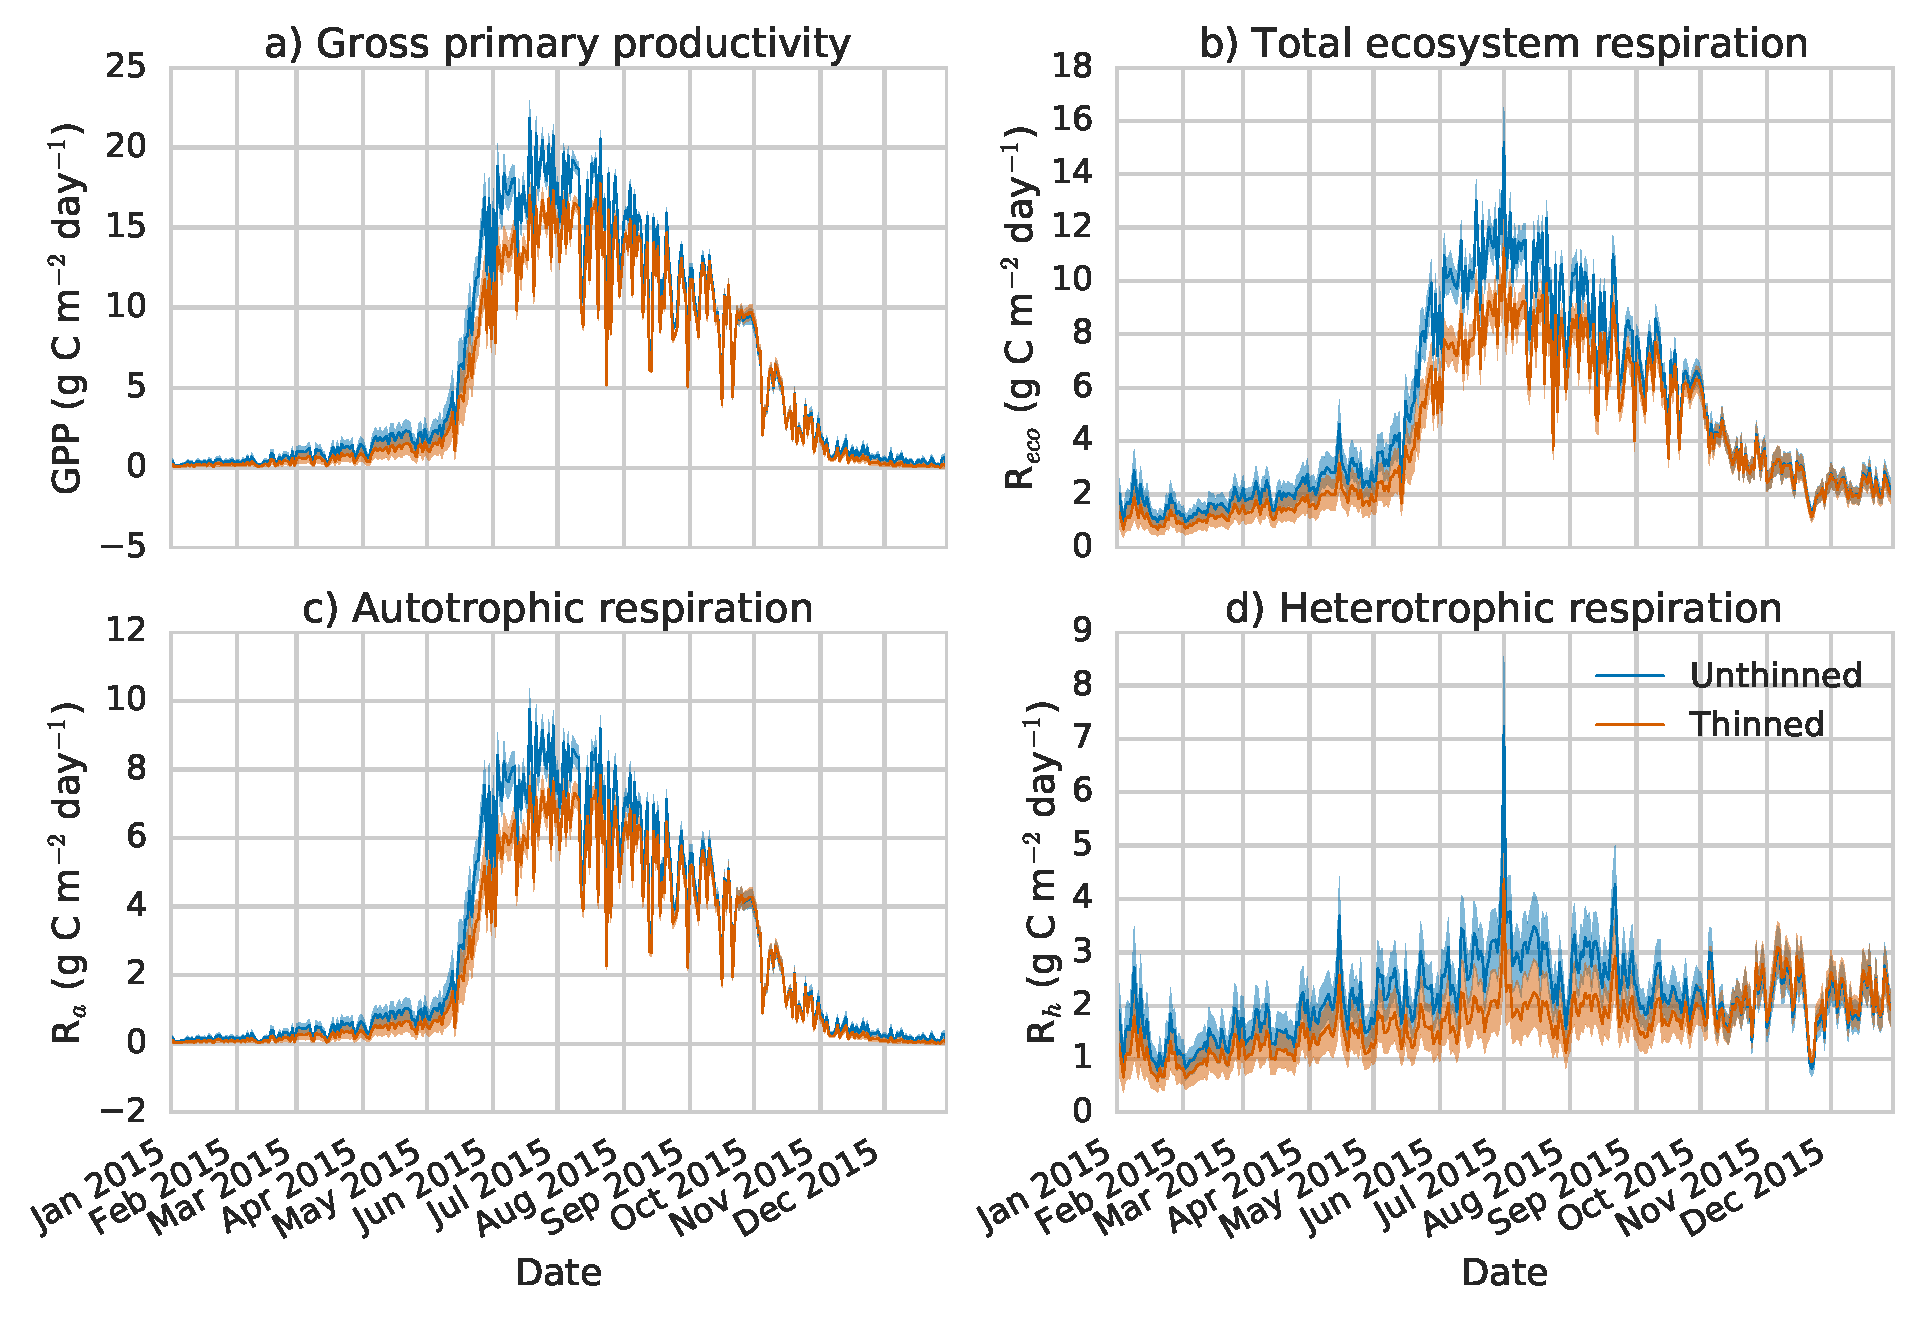
\includegraphics[width=40pc]{flux_compc.pdf}
\caption{Experiment C: 2015 unthinned and thinned forest model trajectories after assimilation. Colour and shading has the same meaning as in Figure~\ref{fig:fluxcompa}.}
 \label{fig:fluxcompc}
 \end{figure}
 
  \begin{figure}
\setfigurenum{S7} %%Change number for each figure
 \noindent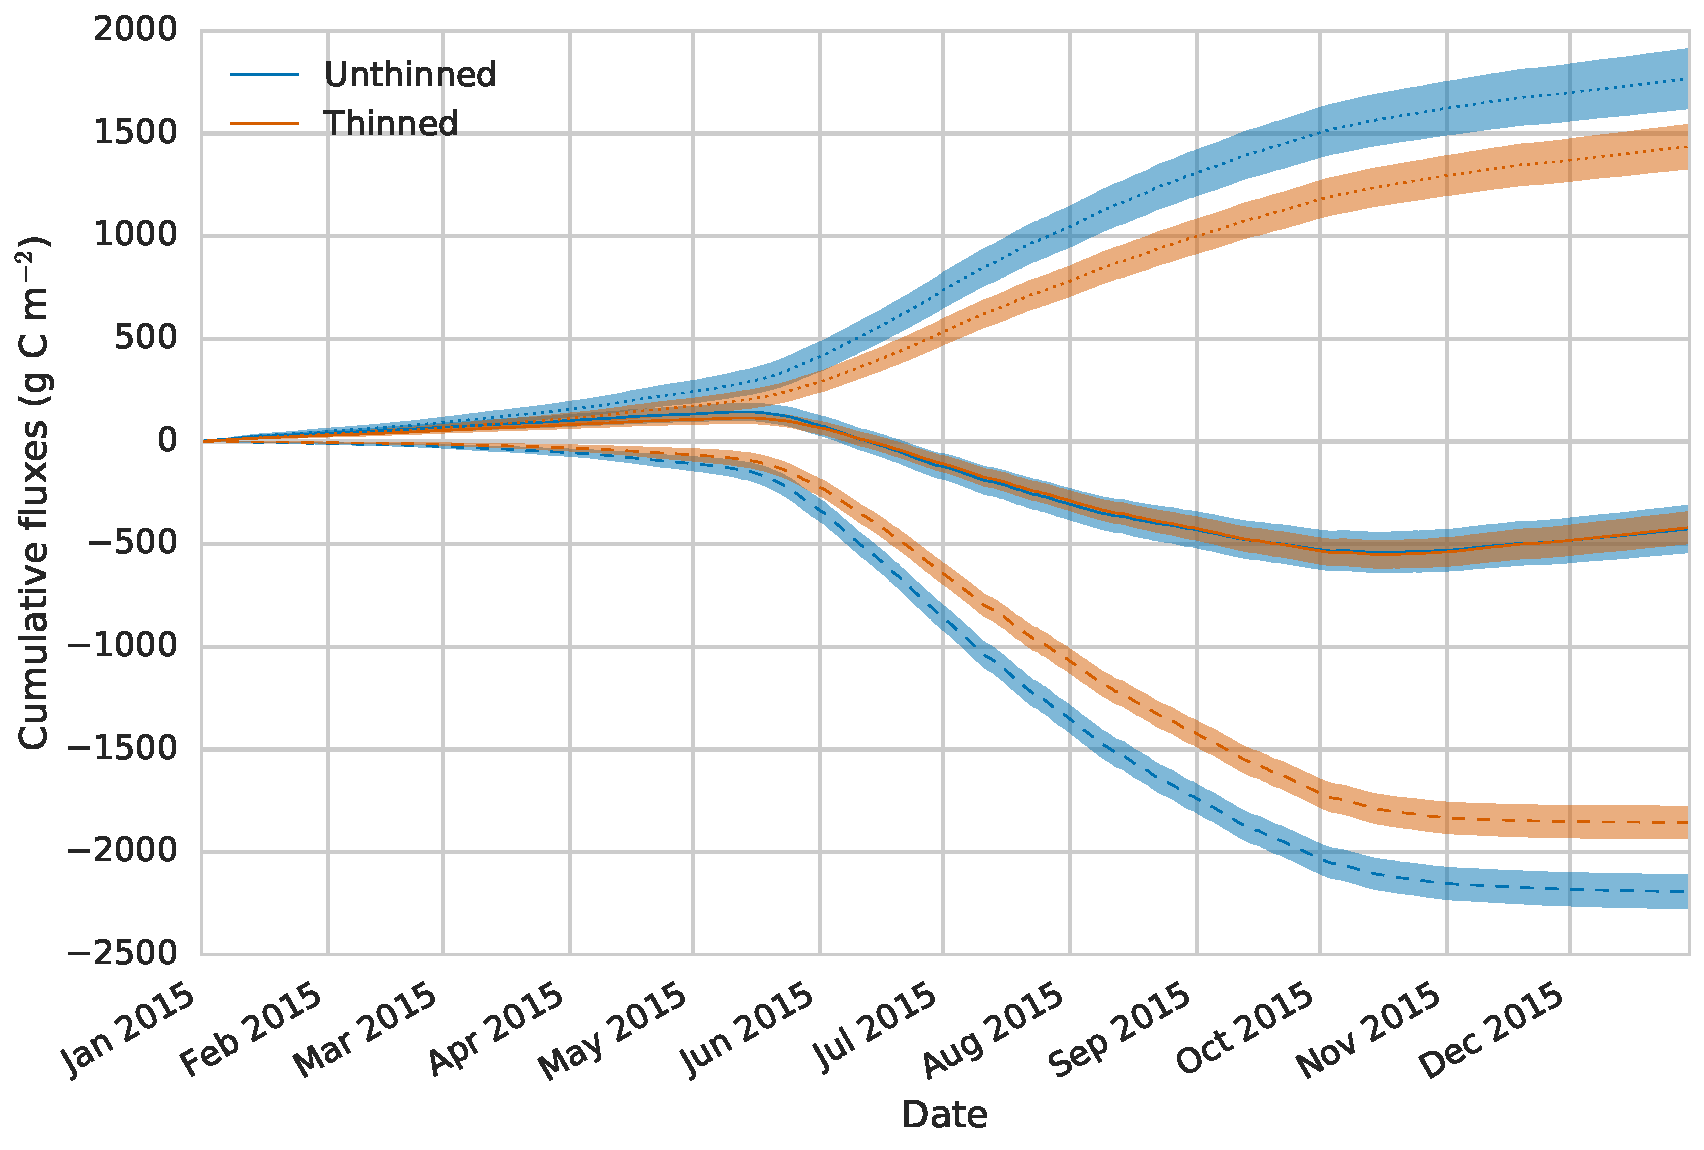
\includegraphics[width=40pc]{cum_fluxc.pdf}
\caption{Experiment C: 2015 unthinned and thinned forest model trajectories for cumulative fluxes after assimilation. Solid line cumulative NEE, dotted line: cumulative ecosystem respiration, dashed line: cumulative GPP (NEE=-GPP+RT). Colour and shading has the same meaning as in Figure~\ref{fig:fluxcompa}.}
 \label{fig:fluxcumc}
 \end{figure}
 
 
  \begin{figure}
\setfigurenum{S8} %%Change number for each figure
 \noindent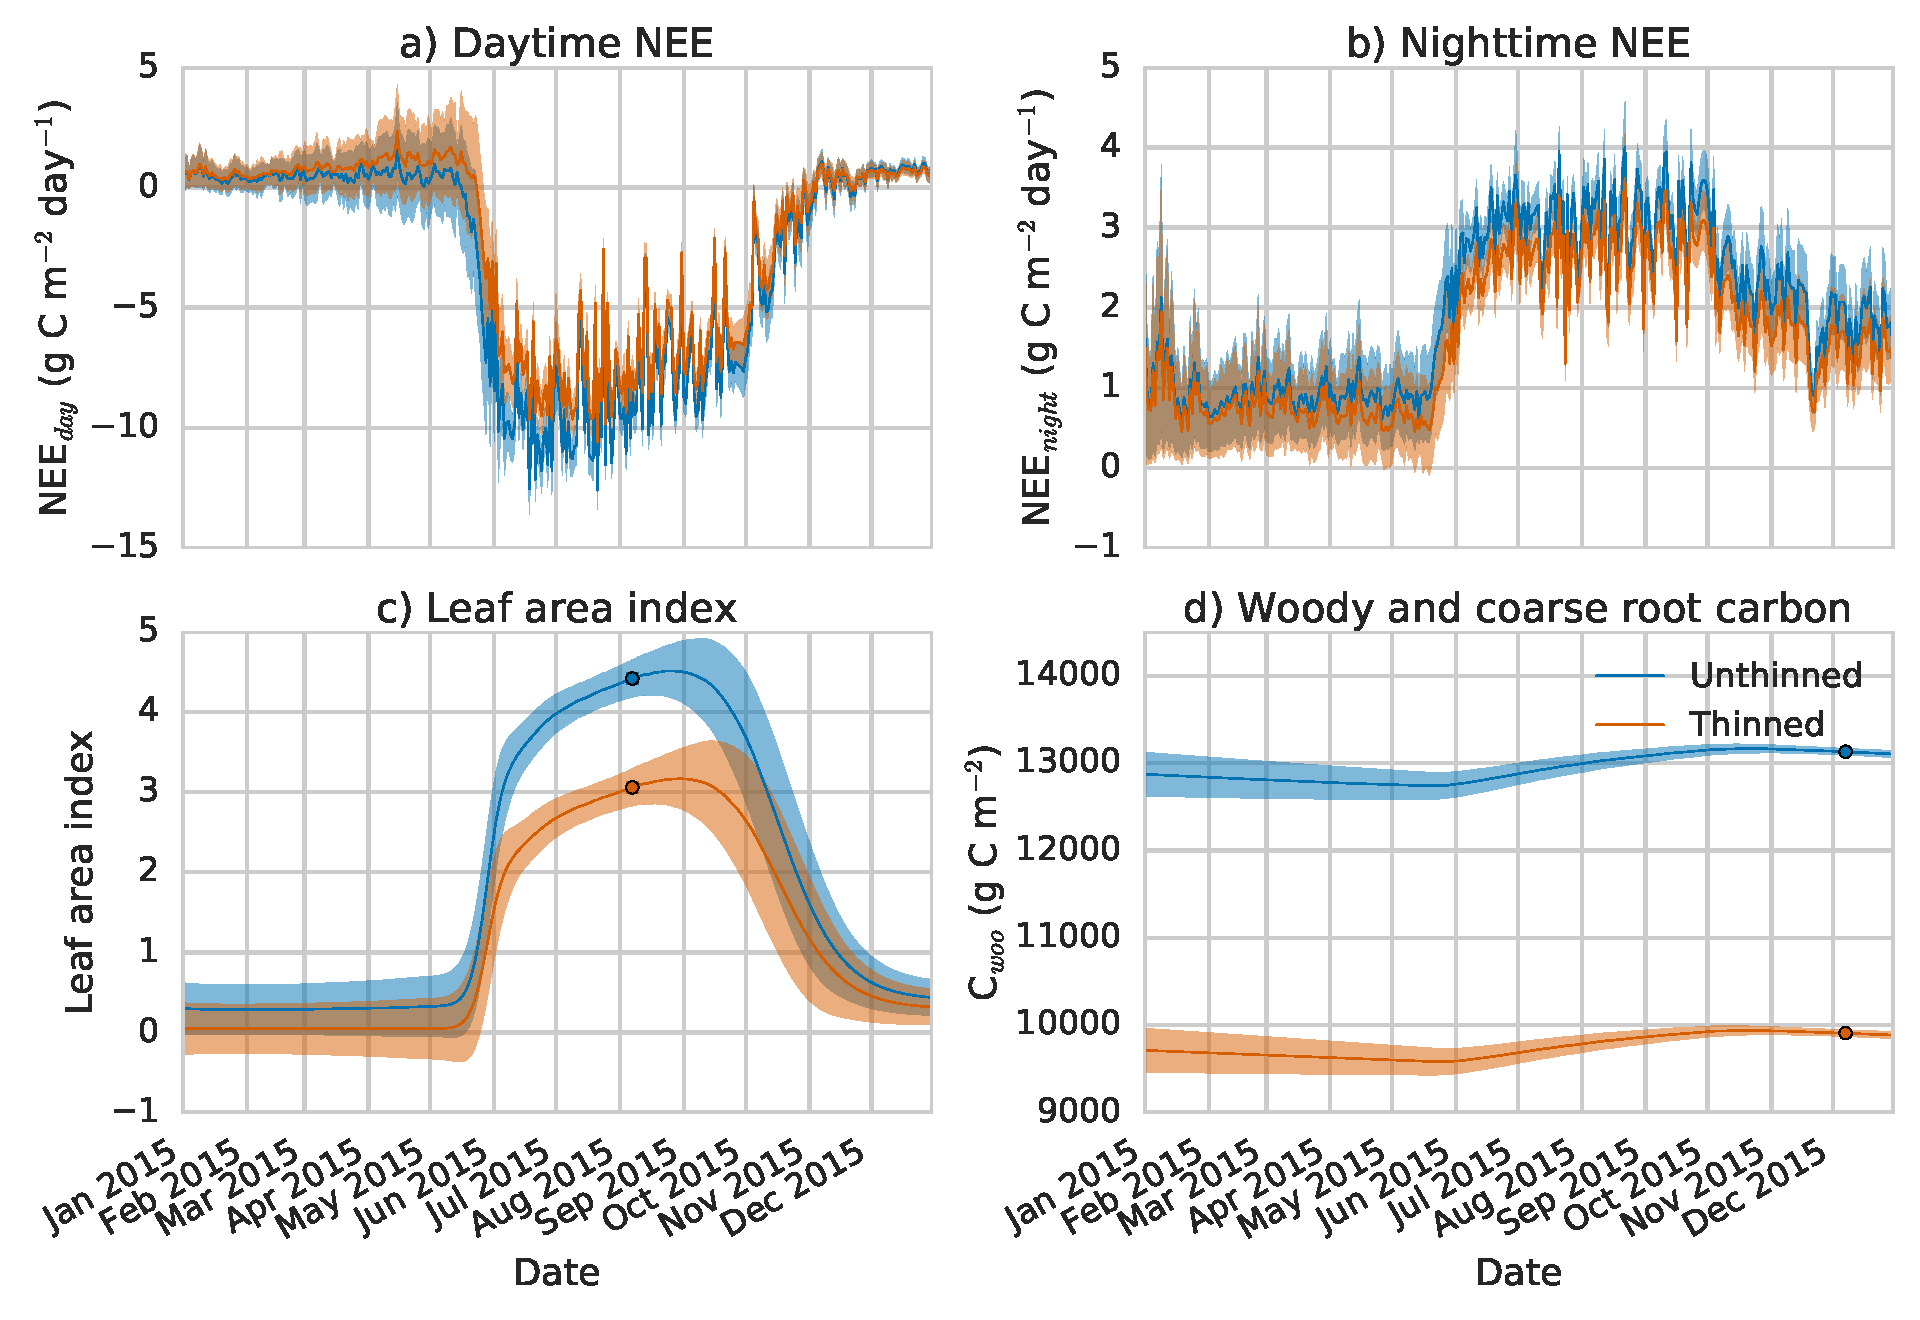
\includegraphics[width=40pc]{obs_compd.pdf}
\caption{Experiment D: 2015 unthinned and thinned forest observations and model trajectories after assimilation. Blue line: model trajectory after assimilation of unthinned data, blue shading: uncertainty in model trajectory after assimilation (\(\pm\) 1 standard deviation), blue dots: unthinned observations with error bars, orange line: model trajectory after assimilation of thinned data, orange shading: uncertainty in model trajectory after assimilation (\(\pm\) 1 standard deviation), orange dots: thinned observations with error bars.}
 \label{fig:obscompd}
 \end{figure}
 
 
 \begin{figure}
\setfigurenum{S9} %%Change number for each figure
 \noindent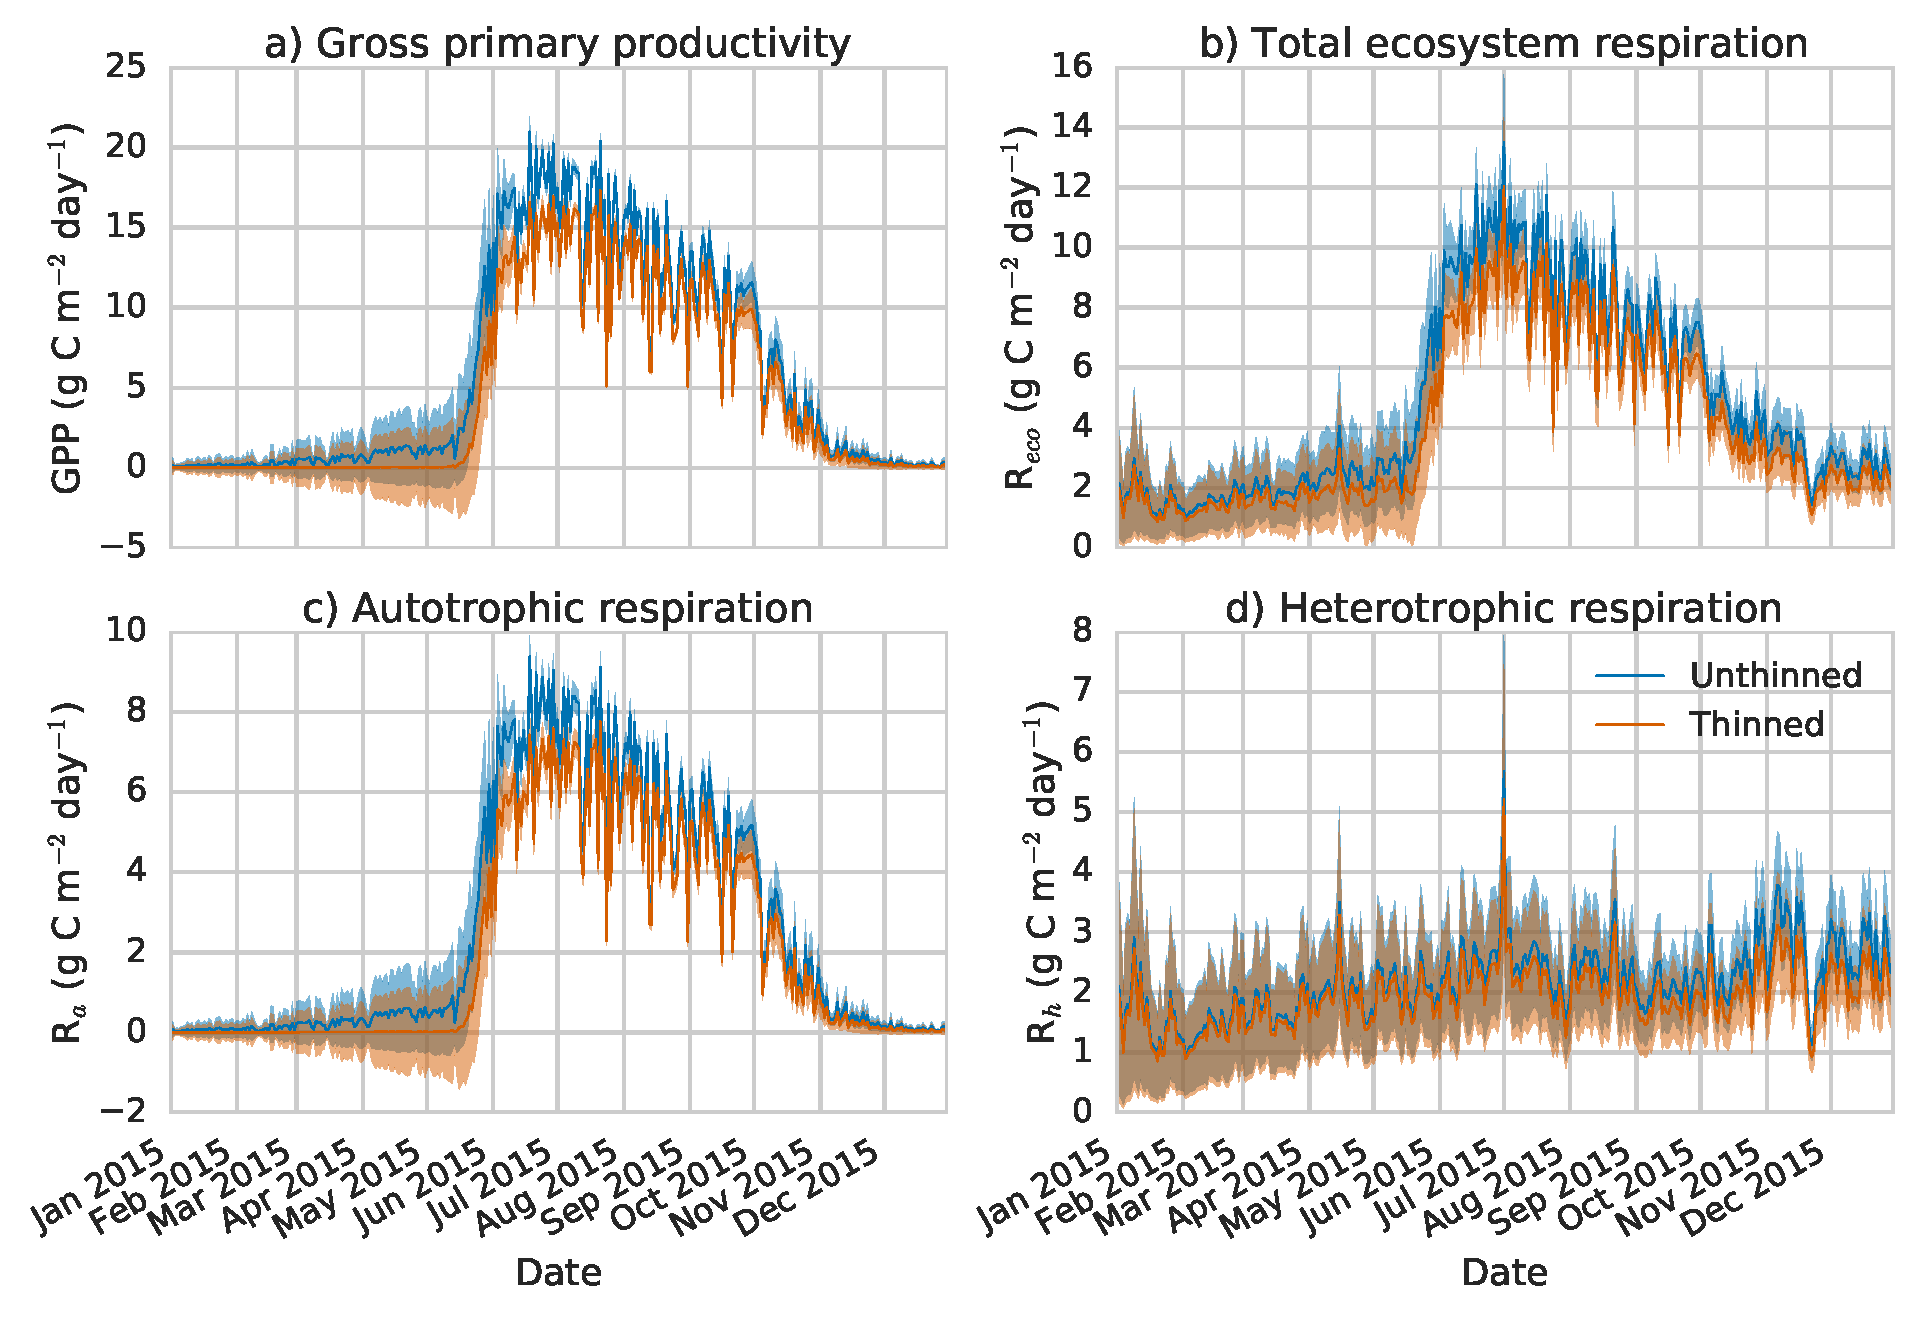
\includegraphics[width=40pc]{flux_compd.pdf}
\caption{Experiment D: 2015 unthinned and thinned forest model trajectories after assimilation. Colour and shading has the same meaning as in Figure~\ref{fig:fluxcompa}.}
 \label{fig:fluxcompd}
 \end{figure}
 
  \begin{figure}
\setfigurenum{S10} %%Change number for each figure
 \noindent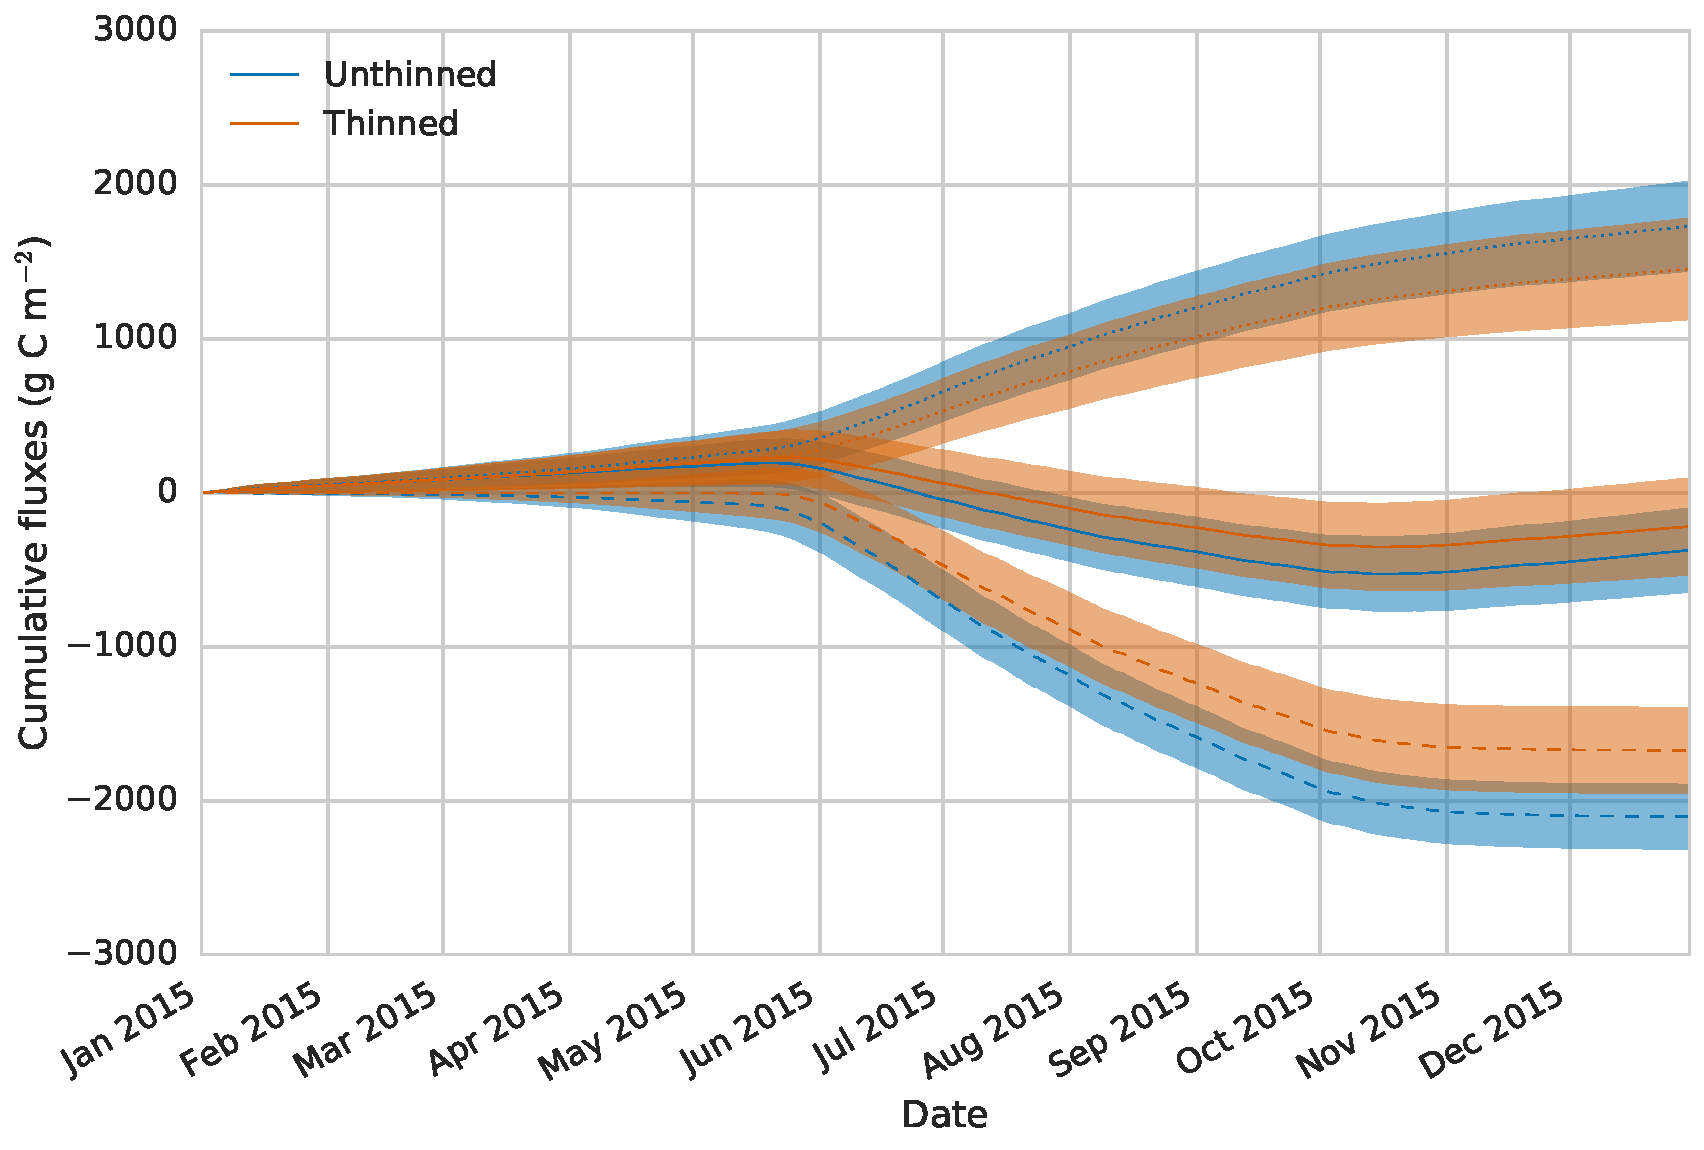
\includegraphics[width=40pc]{cum_fluxd.pdf}
\caption{Experiment D: 2015 unthinned and thinned forest model trajectories for cumulative fluxes after assimilation. Solid line cumulative NEE, dotted line: cumulative ecosystem respiration, dashed line: cumulative GPP (NEE=-GPP+RT). Colour and shading has the same meaning as in Figure~\ref{fig:fluxcompa}.}
 \label{fig:fluxcumd}
 \end{figure}
 
 
 \begin{figure}[ht]
\setfigurenum{S11} %%Change number for each figure
 \noindent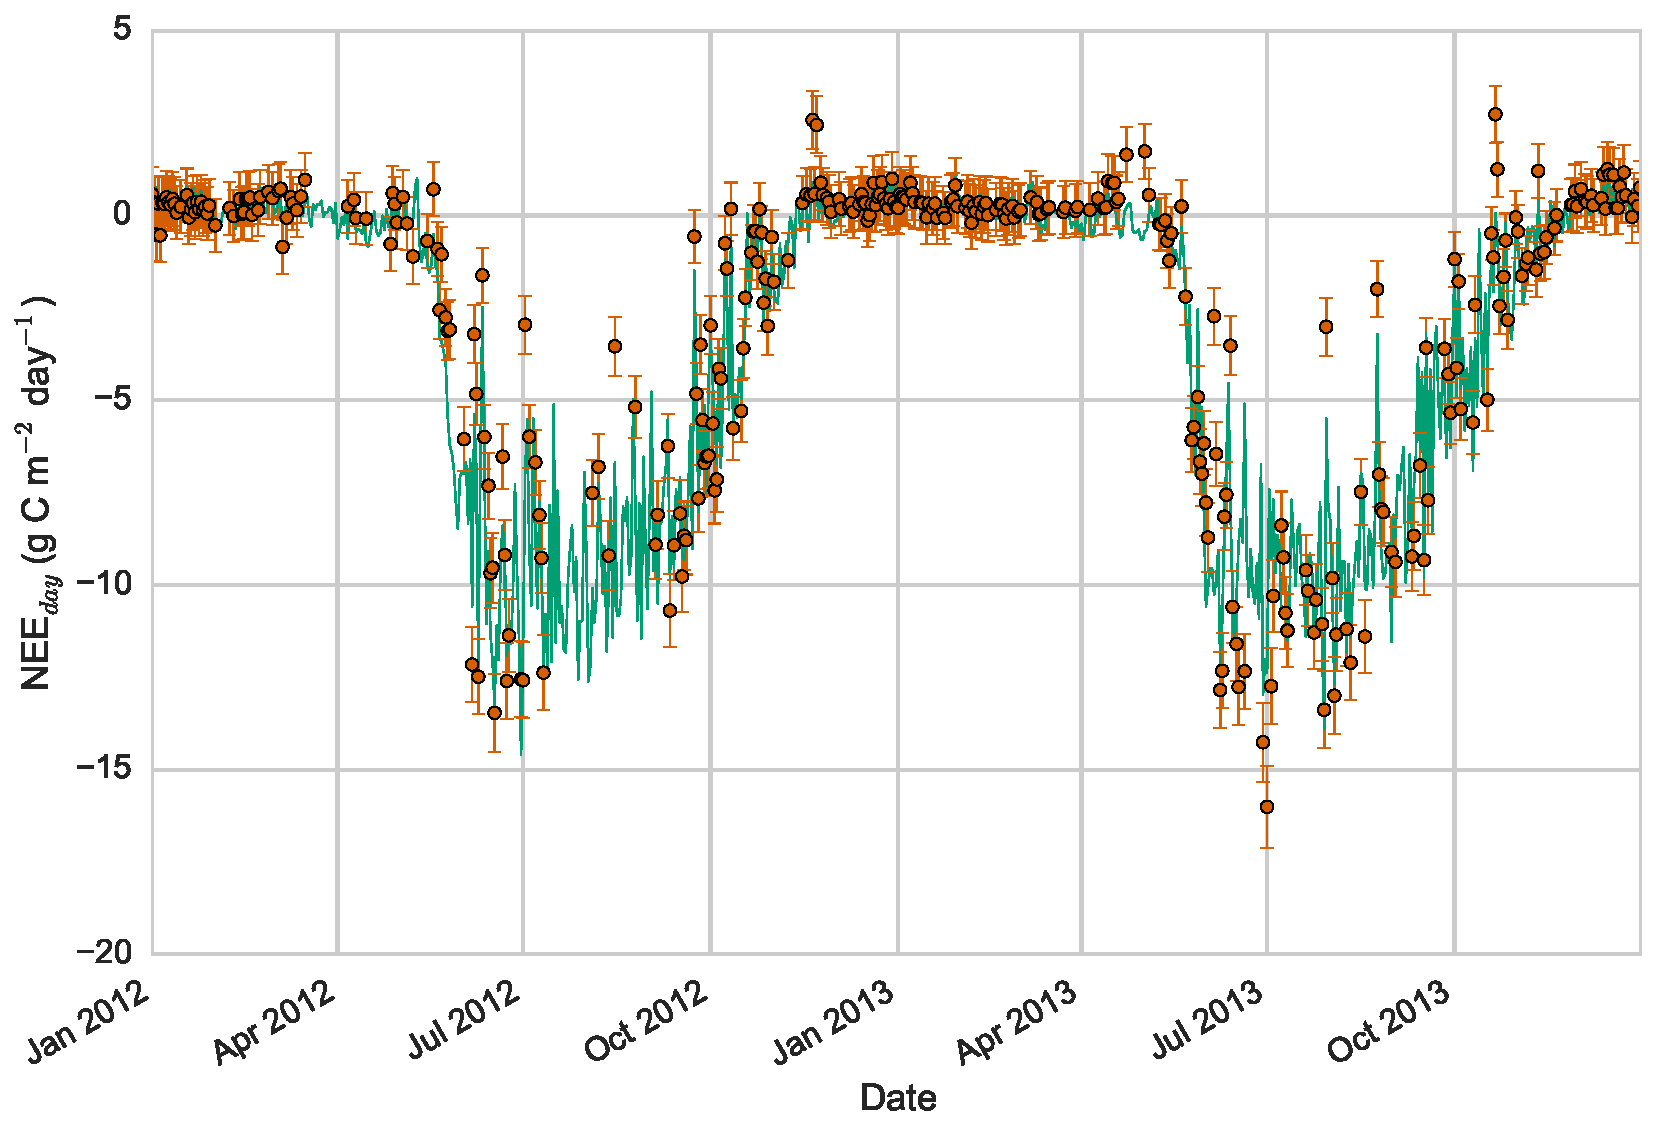
\includegraphics[width=40pc]{prior.pdf}
    \caption{Prior model prediction and observations of daytime NEE for 2012-2013. Green line: model predicted value, orange dots: observations with error bars. The prior model has a correlation coefficient of 0.96 in this case.} 
    \label{fig:prior_mod}
\end{figure}


\begin{figure}[ht]
\setfigurenum{S12} %%Change number for each figure
 \noindent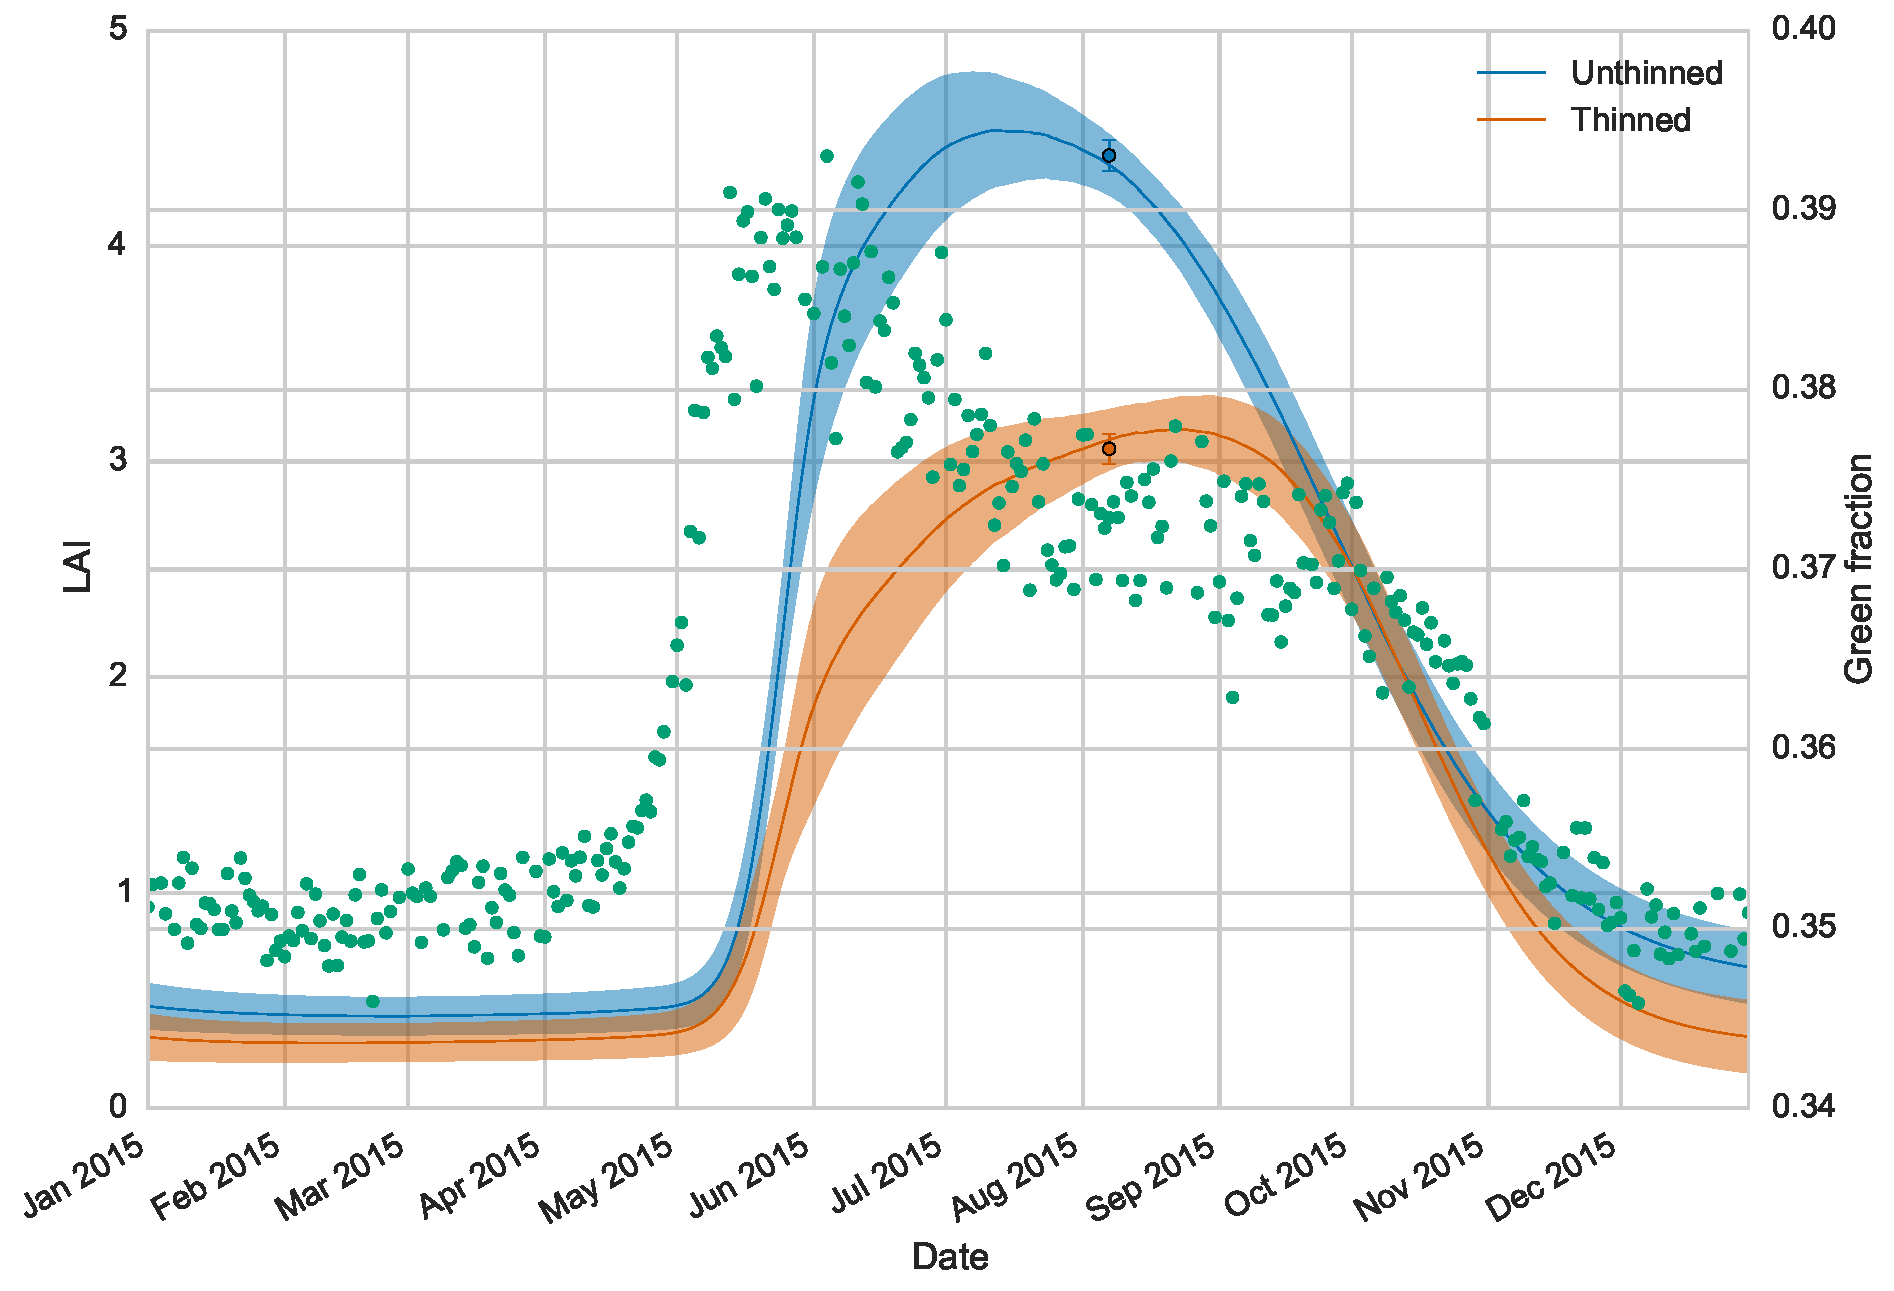
\includegraphics[width=40pc]{pheno_lai.pdf}
    \caption{Model predicted LAI for experiment C and Alice Holt phenocam observations of green fraction (green dots), calculated for the canopy region of interest using red-green-blue digital numbers for each pixel, see \citet{mizunuma2013relationship} for more details.} \label{fig:pheno_obs}
\end{figure}


\begin{figure}[ht]
\setfigurenum{S13} %%Change number for each figure
 \noindent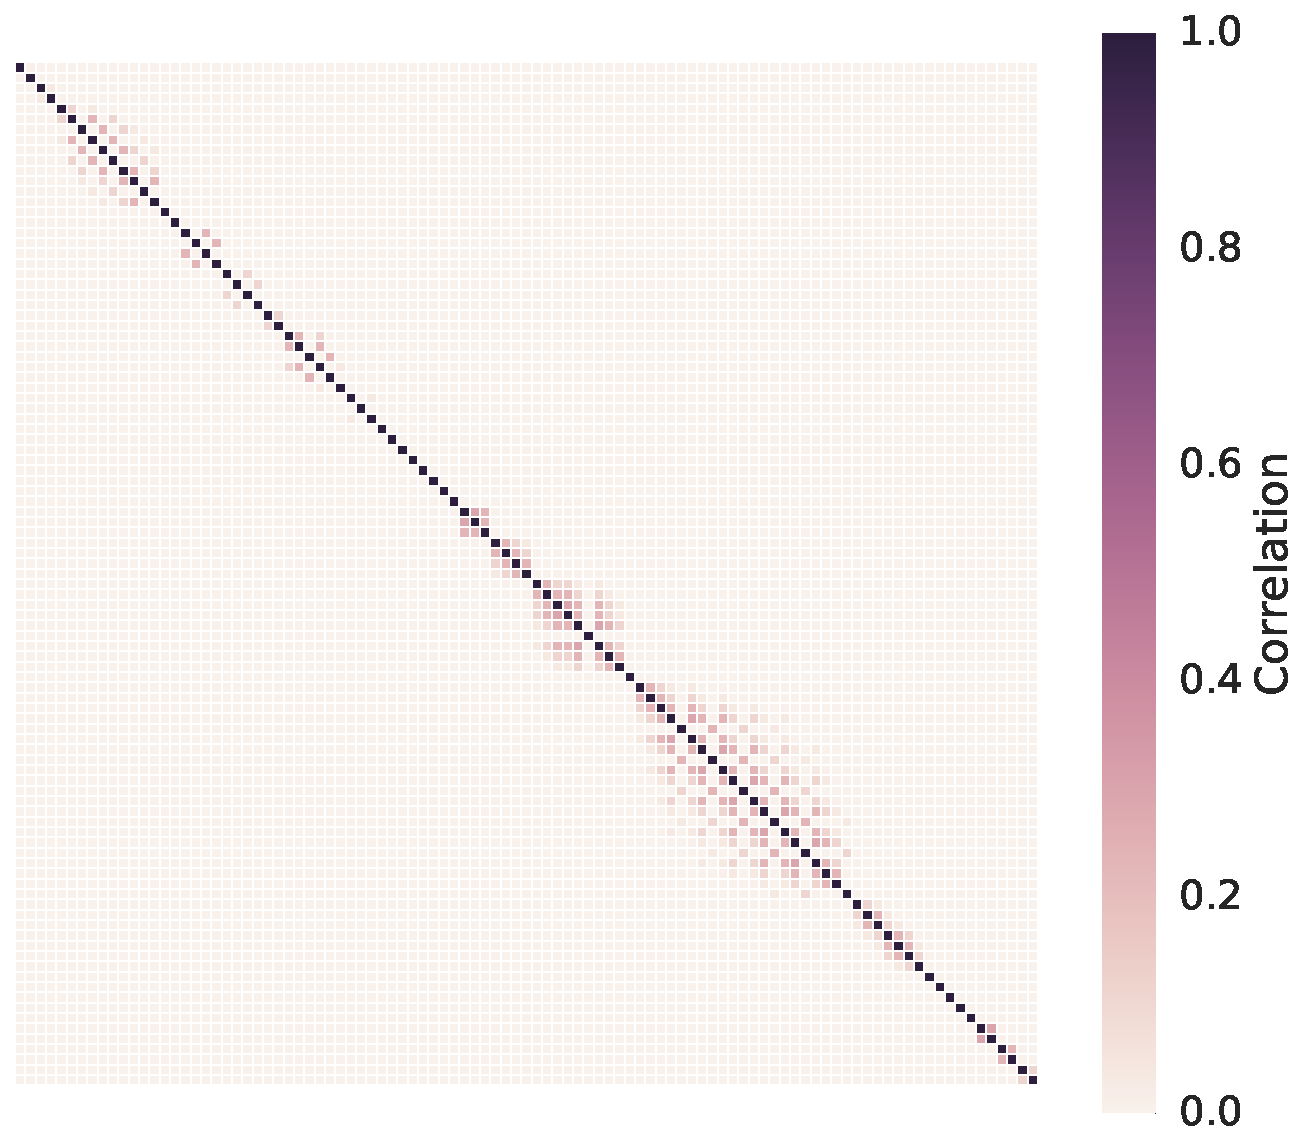
\includegraphics[width=30pc]{rmat_eastc.pdf}
    \caption{Observation error correlation matrix for thinned forest used in experiment C data assimilation. For more details see \citet{Pinnington2016299}.} \label{fig:rmat_ut}
\end{figure}


\begin{figure}[ht]
\setfigurenum{S14} %%Change number for each figure
 \noindent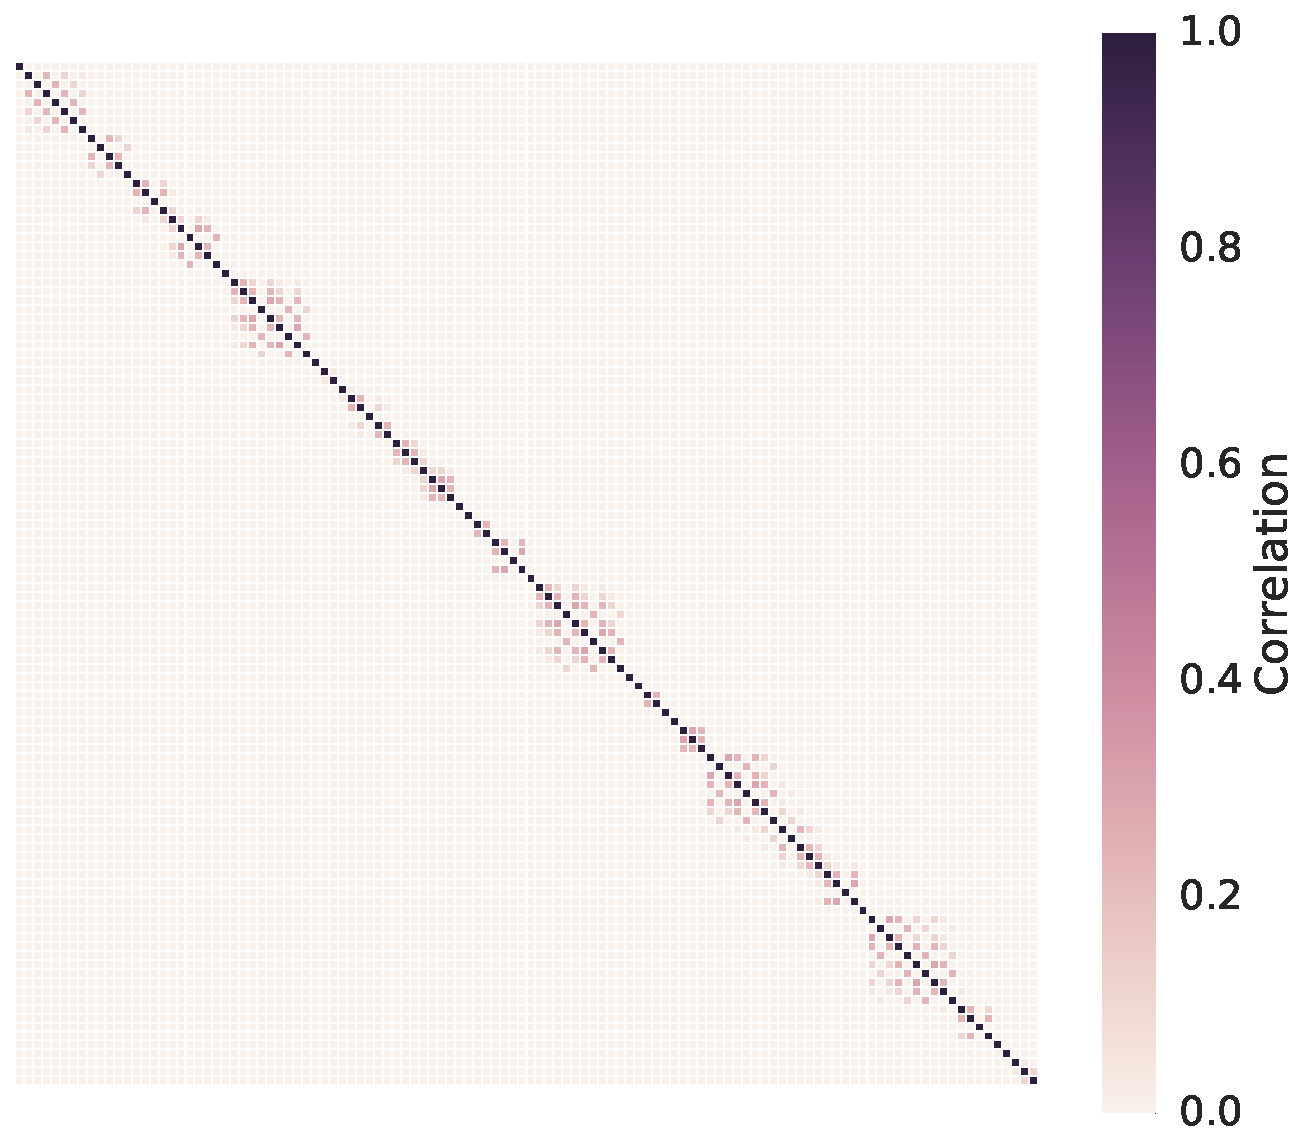
\includegraphics[width=30pc]{rmat_westc.pdf}
    \caption{Observation error correlation matrix for unthinned forest used in experiment C data assimilation. For more details see \citet{Pinnington2016299}.} \label{fig:rmat_t}
\end{figure}
% ---------------
% EXAMPLE TABLE
%
\begin{table}[ht] 
\settablenum{S1}
	\caption{Fit to observations after data assimilation for experiments.}
\begin{center}
	\begin{tabular}{| l | l | l | l | l | l | l | l}
	\hline
	\multicolumn{7}{| c |}{Unthinned side} \\ \hline
	& \multicolumn{2}{| c |}{NEE\(_{day}\)} & \multicolumn{2}{| c |}{NEE\(_{night}\)} & LAI & \(C_{woo}\) \\ \hline
	Exp. & RMSE & \(r^2\) & RMSE & \(r^2\) & RMSE & RMSE  \\ \hline
	A & 0.61 & 0.97 & 0.83 & 0.31 & 2.16 & 6361  \\ \hline
	B & 0.75 & 0.90 & 0.93 & 0.64 & 0.04 & 5987  \\ \hline
	C & 0.75 & 0.90 & 0.93 & 0.64 & 0.04 & 0.16  \\ \hline
	D & 1.22 & 0.74 & 1.00 & 0.89 & 0.0004 & 0.19  \\ \hline
	\multicolumn{7}{| c |}{Thinned side} \\ \hline
	& \multicolumn{2}{| c |}{NEE\(_{day}\)} & \multicolumn{2}{| c |}{NEE\(_{night}\)} & LAI & \(C_{woo}\) \\ \hline
	Exp. & RMSE & \(r^2\) & RMSE & \(r^2\) & RMSE & RMSE  \\ \hline
	A & 0.63 & 0.97 & 0.54 & 0.33 & 0.55 & 2505  \\ \hline
	B & 0.63 & 0.97 & 0.56 & 0.27 & 0.04 & 2241  \\ \hline
	C & 0.63 & 0.97 & 0.56 & 0.27 & 0.04 & 0.07  \\ \hline
	D & 1.24 & 0.88 & 0.60 & 0.17 & 0.001 & 0.07  \\ \hline
	\end{tabular}
	\label{table:sum_stats}
\end{center} 
\end{table}
%\begin{table}
%\settablenum{S1} %%Change number for each table
%\caption{Time of the Transition Between Phase 1 and Phase 2\tablenotemark{a}}
%\centering
%\begin{tabular}{l c}
%\hline
% Run  & Time (min)  \\
%\hline
%  $l1$  & 260   \\
%  $l2$  & 300   \\
%  $l3$  & 340   \\
%  $h1$  & 270   \\
%  $h2$  & 250   \\
%  $h3$  & 380   \\
%  $r1$  & 370   \\
%  $r2$  & 390   \\
%\hline
%\end{tabular}
%\tablenotetext{a}{Footnote text here.}
%\end{table}
% ---------------
%
% EXAMPLE LARGE TABLE (UPLOADED SEPARATELY)
%\begin{table}
%\settablenum{S1} %%Change number for each table
%\caption{Time of the Transition Between Phase 1 and Phase 2\tablenotemark{a}}
%\end{table}


\end{document}

%%%%%%%%%%%%%%%%%%%%%%%%%%%%%%%%%%%%%%%%%%%%%%%%%%%%%%%%%%%%%%%

More Information and Advice:

%% ------------------------------------------------------------------------ %%
%
%  SECTION HEADS
%
%% ------------------------------------------------------------------------ %%

% Capitalize the first letter of each word (except for
% prepositions, conjunctions, and articles that are
% three or fewer letters).

% AGU follows standard outline style; therefore, there cannot be a section 1 without
% a section 2, or a section 2.3.1 without a section 2.3.2.
% Please make sure your section numbers are balanced.
% ---------------
% Level 1 head
%
% Use the \section{} command to identify level 1 heads;
% type the appropriate head wording between the curly
% brackets, as shown below.
%
%An example:
%\section{Level 1 Head: Introduction}
%
% ---------------
% Level 2 head
%
% Use the \subsection{} command to identify level 2 heads.
%An example:
%\subsection{Level 2 Head}
%
% ---------------
% Level 3 head
%
% Use the \subsubsection{} command to identify level 3 heads
%An example:
%\subsubsection{Level 3 Head}
%
%---------------
% Level 4 head
%
% Use the \subsubsubsection{} command to identify level 3 heads
% An example:
%\subsubsubsection{Level 4 Head} An example.
%
%% ------------------------------------------------------------------------ %%
%
%  IN-TEXT LISTS
%
%% ------------------------------------------------------------------------ %%
%
% Do not use bulleted lists; enumerated lists are okay.
% \begin{enumerate}
% \item
% \item
% \item
% \end{enumerate}
%
%% ------------------------------------------------------------------------ %%
%
%  EQUATIONS
%
%% ------------------------------------------------------------------------ %%

% Single-line equations are centered.
% Equation arrays will appear left-aligned.

Math coded inside display math mode \[ ...\]
 will not be numbered, e.g.,:
 \[ x^2=y^2 + z^2\]

 Math coded inside \begin{equation} and \end{equation} will
 be automatically numbered, e.g.,:
 \begin{equation}
 x^2=y^2 + z^2
 \end{equation}

% IF YOU HAVE MULTI-LINE EQUATIONS, PLEASE
% BREAK THE EQUATIONS INTO TWO OR MORE LINES
% OF SINGLE COLUMN WIDTH (20 pc, 8.3 cm)
% using double backslashes (\\).

% To create multiline equations, use the
% \begin{eqnarray} and \end{eqnarray} environment
% as demonstrated below.
\begin{eqnarray}
  x_{1} & = & (x - x_{0}) \cos \Theta \nonumber \\
        && + (y - y_{0}) \sin \Theta  \nonumber \\
  y_{1} & = & -(x - x_{0}) \sin \Theta \nonumber \\
        && + (y - y_{0}) \cos \Theta.
\end{eqnarray}

%If you don't want an equation number, use the star form:
%\begin{eqnarray*}...\end{eqnarray*}

% Break each line at a sign of operation
% (+, -, etc.) if possible, with the sign of operation
% on the new line.

% Indent second and subsequent lines to align with
% the first character following the equal sign on the
% first line.

% Use an \hspace{} command to insert horizontal space
% into your equation if necessary. Place an appropriate
% unit of measure between the curly braces, e.g.
% \hspace{1in}; you may have to experiment to achieve
% the correct amount of space.


%% ------------------------------------------------------------------------ %%
%
%  EQUATION NUMBERING: COUNTER
%
%% ------------------------------------------------------------------------ %%

% You may change equation numbering by resetting
% the equation counter or by explicitly numbering
% an equation.

% To explicitly number an equation, type \eqnum{}
% (with the desired number between the brackets)
% after the \begin{equation} or \begin{eqnarray}
% command.  The \eqnum{} command will affect only
% the equation it appears with; LaTeX will number
% any equations appearing later in the manuscript
% according to the equation counter.
%

% If you have a multiline equation that needs only
% one equation number, use a \nonumber command in
% front of the double backslashes (\\) as shown in
% the multiline equation above.

%% ------------------------------------------------------------------------ %%
%
%  SIDEWAYS FIGURE AND TABLE EXAMPLES
%
%% ------------------------------------------------------------------------ %%
%
% For tables and figures, add \usepackage{rotating} to the paper and add the rotating.sty file to the folder.
% AGU prefers the use of {sidewaystable} over {landscapetable} as it causes fewer problems.
%
% \begin{sidewaysfigure}
% \includegraphics[width=20pc]{samplefigure.eps}
% \caption{caption here}
% \label{label_here}
% \end{sidewaysfigure}
%
%
%
% \begin{sidewaystable}
% \caption{}
% \begin{tabular}
% Table layout here.
% \end{tabular}
% \end{sidewaystable}
%
%

